\documentclass[twocolumn]{article}
\title{Integrated distributed optimization of IoT service placement and traffic routing}
\date{\today}
\usepackage{cite}
\author{Evangelos Pournaras, Zeinab Nezami}
\usepackage{lipsum}
%\usepackage[landscape]{geometry}
%\usepackage{lscape}
\usepackage{multicol}
\usepackage{amsmath,amssymb,amsfonts}
\usepackage{enumitem}
\usepackage{algorithm,algpseudocode}
\usepackage{xcolor}
\usepackage{graphicx}
\usepackage{setspace}
\usepackage{caption}
\usepackage{subcaption}
\usepackage{supertabular}
\usepackage{multirow}
\usepackage[perpage,hang,flushmargin]{footmisc}
\newcommand{\abbrlabel}[1]{\makebox[3cm][l]{\textbf{#1}\ \dotfill}}
\newenvironment{abbreviations}{\begin{list}{}{\renewcommand{\makelabel}{\abbrlabel}}}{\end{list}}

%-----------------------------------
%from EPOS TEMPLATE ARE COPIED HERE:
%-----------------------------------

%% common abbreviations
%\newcommand{\ie}{i.e.,\xspace}
%\newcommand{\eg}{e.g.\xspace}
%\newcommand{\Ie}{I.e.,\xspace}
%\newcommand{\Eg}{E.g.\xspace}
%\newcommand{\etal}{\emph{et.\ al.\ }\xspace}
%\newcommand{\des}[1]{\mbox{\scriptsize #1}}
%\newcommand{\vect}[1]{\boldsymbol{#1}}

% A set depicted with bold:
%\newcommand{\set}[1]{\ensuremath{\mathbf{#1}}\xspace}

% The elements of a set:
%\newcommand{\elements}[3]{\ensuremath{\{#1_{#2},...,#1_{#3}\}}%\xspace}

%The cardinality of a given set belonging somewhere:
%\newcommand{\cardinality}[2]{\ensuremath{|\set{#1}_{#2}|}%\xspace} 		

% A mathematical unit:
%\newcommand{\unit}[1]{\ensuremath{\mathrm{#1}}\xspace} 	

%\DeclareMathOperator*{\argmin}{arg\,min}

%\newtheorem{definition}{Definition}

\begin{document}

\maketitle

%\renewcommand{\baselinestretch}{1}

\section{Introduction}
\par Joint distributed optimization
\par In 2019, the UK domestic transport was responsible for emitting 122 MtCO2e (million tonnes of carbon dioxide equivalent) which makes it the largest emitting sector of greenhouse gas (GHG) emissions, producing 27\% of the
UK's total emissions. Reflected by International Energy Agency (IEA)\footnote{https://www.iea.org/data-and-statistics/charts/transport-sector-co2-emissions-by-mode-in-the-sustainable-development-scenario-2000-2030, last accessed July 2022}, the entire transport sector accounts for 21\% of total emissions from which road travel accounts for three-quarters of transport emissions. Most of this comes from passenger vehicles (e.g., cars and buses) which contribute 45.1\%. The other 29.4\% comes from trucks carrying freight. Congestion does more than waste time and resources, it adds to localized pollutants. Policy makers have placed less attention on reducing CO2 emissions by reducing traffic congestion. As traffic congestion increases, so too do fuel consumption and CO2 emissions\footnote{Transport energy and environment statistics, accessed August 2021, https://www.gov.uk/government/statistics/transport-and-environment-statistics-2021}.

\par At the same time, with the rapid advancements in Intelligent Transportation Systems (ITS) technologies such as Internet of Vehicles (IoV), connected and autonomous vehicles (AV) are envisioned to provide a safer, greener\cite{ligo2017throughput,cheng2018planning} and much more convenient\cite{chen2017service,silva2018ethical} transportation system for the public. Vehicles are equipped with wireless communication capabilities for both intra-vehicle and inter-vehicle communications to support a plethora of applications including those for traffic control, road safety, smart transportation, and location-dependent services\cite{lu2014connected,lin2017resource}.

\par International Data Corporation (IDC) report estimates that there will be 41.6 billion Internet of Things (IoT) devices including vehicles in 2025 with a potential of generating up to 79.4 zettabytes (ZB) of data\cite{gantz2019digitization}. 
Energy consumption of information and communications technology (ICT) is already accounting for more
than 10\% of global energy consumption and is expected to exceed the 20\% mark by 2030\cite{jones2018stop}. While worldwide energy consumption has significantly dropped as a result of global lockdown restrictions, Internet usage has seen a huge spike, particularly in use of bandwidth-intensive and delay sensitive application.

\par Due to the resource-limited on-board computers of vehicles, many potential applications, such as assistant accident
avoidance\cite{rani2016computer,priyanka2017sudden}, mobile crowd sensing\cite{chen2018survey} and augmented reality\cite{rameau2016real}, which require significant computing power to process data generated by the vehicle sensors in a real-time fashion\cite{lee2015development}, pose a grand challenge to vehicular terminals.
The general trend of cloud computing is a straightforward solution for processing such an amount of data. However, in certain scenarios such as autonomous cars and interactive wearable cognitive assistance applications with strict latency requirements the latency introduced by unstable connections and transmitting heavy payloads from/to the cloud can be prohibitive\cite{tarneberg2017dynamic,chen2018application,montero2017extending,byers2017architectural,chen2017empirical,azizi2019priority,ha2013impact}. 

\par By shifting the cloud services to the network edges such as the radio access network, fog computing (FC)\cite{bonomi2014fog,li2019energy} and mobile-edge computing (MEC) provide a new paradigm to offload computation from cloud to local fog servers (LFSs) or MEC  servers while at the same time allow for the use of IoT services with location awareness and mobility support to make up for the disadvantages of cloud computing\cite{satria2017recovery}.. Vehicular Edge Computing (VEC) has been widely discussed in the literature\cite{bitam2015vanet,abdelhamid2015vehicle}, where the computing infrastructures at both the network and the vehicles are used by mobile users. If performed suitably, service offloading reduces the energy consumption and speeds up the response time of applications in a VEC scenario\cite{zhang2014collaborative,lyu2016multiuser,wang2017computation}.
This paper studies the utilization of FC resources not limited to the MEC but along an edge-to-cloud continuum to address data-intensive and low latency requirements of vehicular services, as well as to avoid the bottlenecks of centralized servers.

\par Research also has shown that distributed architectures of MEC and FC could save between 14\% to more than 80\% of total energy consumption compared to fully centralized architectures of cloud data centers\cite{ahvar2019estimating,yan2019modeling}. By reducing the amount of data traversing the network, FC could lead to a significant reduction in energy consumption and carbon emissions. 
Nevertheless, the distributed and resource-constrained nature of fog infrastructure (especially in terms of battery power) raise challenges regarding its capability of hosting numerous diverse services: (i) Unlike the cloud, these nodes cannot scale infinitely to host always-running Virtual Machines (VM) and containers, while an overloaded edge server significantly degrades user experience and negates the advantages of FC\cite{satria2017recovery,baresi2017empowering}.
(ii) Due to the dynamicity of the environment, mobile devices may appear and disappear, others are moving, and application information may change over time (e.g., the variation of the workload).  (iii) Due to the randomness of service arrivals, vehicles always have a tendency to choose edge servers for offloading in a selfish way, which is not satisfactory for the social good of the whole system and even results in a failure possibility of some services due to the overflow of some servers\cite{li2019compound}. (iv) Cost-related factors become very influential in fog service management, from both users' and service provider's point of view. 

\par As a matter of fact, the major obstacle to adopting FC is how to efficiently deploy services on available edge-to-cloud resources\cite{salaht2020overview,nezami2021decentralized}, i.e, service placement, which is a multi-constrained NP-hard problem\cite{brogi2017,bokhari1981mapping}. Running all application requests at the edge nodes near road intersections or vehicles' destinations where a larger number of vehicles are present may make some of the nodes overloaded. In addition to workload balance, with mobile users/vehicles and their inherent traffic dynamics, real-time interaction and energy saving are also critical\cite{salaht2020overview,nezami2021decentralized,colistra2015task,brogi2017,yousefpour2019fogplan,he2013mobility,luan2013engineering,lu2014connected}.
As a result, further to Quality of Service (QoS) parameters, different optimization aspects come into account\cite{salaht2020overview,yousefpour2019all} to solve the service placement problem including.

\par While distributed control plane helps to address centralized approaches vulnerabilities regarding single point of failure, scalability and computational complexity issues, it also provides locality awareness, enhanced resource utilization, and can be more efficient to handle the dynamic changes of infrastructure like fog\cite{salaht2020overview,nezami2021decentralized}. Therefore, this paper studies a fully decentralized management strategy which explores the trade-off between power consumption, service delay, and workload balance in the fog-cloud computing system.

\par Our validation scenario targets the Vehicle to Infrastructure (V2I) communication model and benefits the networking and computation nodes along the Edge-to-Cloud hierarchy as its infrastructure. In particular, we focus on video streams from
vehicles' cameras that need to be analyzed for object detection, tracking, and navigating AVs. In this particular case, as it is often the case with IoT applications, a high QoS level is required. Indeed, data lose their
value when they cannot be analyzed fast enough.

\subsection{Motivating Example}
%\par The US National Highway Transportation Safety Administration (NHTSA) found that more than 90\% of vehicle accidents are caused by driver errors. Safe driving requires drivers to process large amounts of dynamic information under time pressure. However, drivers can attend to only a small percentage of visual stimuli at once.

\par The auto industry is racing to build technologies that will lead to fully driverless cars. In 2025, the global automotive AR and virtual reality (VR) market is forecast to reach about \$673bn, up from \$0.21bn in 2017 \footnote{https://www.vanarama.com/car-leasing/blog/4-ways-augmented-reality-will-revolutionise-the-automotive-industry.html}. It's not just Google: Ford, BMW, Tesla, General Motors and others are all investing in Civil Maps\footnote{https://civilmaps.com/} to develop 3D high-resolution maps to bring fully AVs a step closer to reality. The Localization and AR Maps provide a self-learning cognitive perception system that replicate human context to enable machines to perceive, orient and respond to the physical world in real-time.
\par What Civil Maps wants to do is to create a Waze for driverless cars, one that builds a picture of everything from traffic patterns to construction zones. Using a package of hardware and software, cars equipped with Civil Maps' technology will be able to read street signs, traffic lights and warnings, then compress that data and upload it over a cellular connection.
The application turns every commuter into a data-gatherer to continuously update maps for AVs: It lets vehicles report traffic jams, crashes and other issues that pose a danger or delay to others, resulting in a crowd-sourced map, accurate to the nearest three to five centimeters that anyone can read. 

\par Machines are allowed to crowd-source data from many vehicles and connect to the \textbf{cloud} through 4G LTE for automated data collection and mapping process. The infrastructure might be changing on a daily or weekly basis, while up to now, most online mapping data is only updated every few months at best because it's too expensive to upload that data wirelessly. This is part of the reason why self-driving cars aren't ready yet for prime time, said Puttagunta (Civil Maps co-founder Sravan Puttagunta). Now consider the following two situations that need instantaneous updates and notifications in different space scales:

\begin{enumerate}
\item A leading vehicle encounters an unexpected pothole and wants to notify its following cars to avoid a potential
accident. Real-time latency, street scale.
\item Congested traffic is out of sight for cars planning to take a road on their right side. Vehicles in the congestion
broadcast to all the network so that cars can compute another optimal itinerary. Medium latency, city scale.
\end{enumerate}

\par Current V2V or V2C architectures and solutions cannot handle these scenarios due to the diversity of the requirements.
In V2C, the combined latency of transmission, processing, and distribution prevents emergency updates and decisions to be propagated on time. On the other hand, although V2V significantly improves performance at close distance, forwarding information at city scale is inefficient and costly. Finally, V2I provides better data distribution. However, sharing accurate emergency information entails nontrivial computation and coordination in a limited amount of time. Edge-Cloud infrastructures should therefore integrate computing features for fast and reliable emergency map updates and propagation.

\par Motivated by the above-mentioned scenarios, and the dynamic and time-variant characteristics of the vehicular environment, we propose to leverage the edge-to-cloud infrastructure to study the energy consumption, service delay, and workload balance trade-offs in running AR services using distributed placement algorithms in such an environment.

\section{Service Placement Problem}
\par Mobile data that requires high computing power will grow rapidly in the coming years, driven mainly by mobile video streaming and the IoT. The processing capabilities and storage capacities of the cloud servers are higher than those of the edge servers. However, the edge servers ensure low latency, enabling real-time processing. This is due to the proximity between edge and mobile devices (e.g., vehicles). Considering the processing and latency trade-offs between edge and cloud, a placement planning algorithm is required which is the focus of this paper. 

\subsection{System Model}
\par This paper tailors the system proposed in our previous work\cite{nezami2021decentralized} to provide mobility support for IoT service placement in vehicular networks and ??.... This work envisions an edge-to-cloud infrastructure consisting of I = {1, 2, ... , i} vehicles, a set of P = {1, 2, ... , p} cellular base stations (Access Points (AP) from now on) such that i < p, edge and core routers, servers, and the central cloud as shown in Fig\ref{fig:system}. The network involves bidirectional traffic flow. We consider vehicles to be equipped with a cellular radio interface\cite{malandrino2013content}. APs are equipped with 4G LTE modules connecting them to the core/cloud nodes via Wide Area Network. A vehicle can be connected maximum to one AP at once and APs are connected with each other through wireless backhauls. 

\par The coverage range of APs is overlapping while covering the entire area. The APs collect data from vehicles and send it to their connected server for storage/processing. With the computational and storage units, named fog servers, optionally co-located with the APs and routers the network allows to reduce the overall latency compared to vehicle-to-cloud and significantly trim the complexity of vehicle-to-vehicle communication. 
Network devices include routers and switches between the APs and the cloud. We assume that the local servers are linked to the access points through edge routers while the cloud is reached through core routers. The edge servers closer to vehicles can serve latency-sensitive applications such as emergency notifications while those co-located with core routers may be used for map updates.

\par In our scenario driverless vehicles represent IoT devices with a continuously running AR application, each of them may has a different data generation rate. As a result, the time taken to execute a service depends on the data rate and the available computing capacity of the server to which it is assigned. We select an in-vehicle IoT device (e.g., HUD, smart rearview mirror) as our client device that needs provide object detection services. Any vehicle demanding AR services sends a connection request, characterized by several parameters listed in table\ref{tab:notation}, together with its basic information (e.g., camera image, IP, profile, velocity, timestamp, the orientation of the vehicle, and GPS coordinates) to its communicating fog server (connecting AP when the vehicle meets with the AP) for execution. Fog servers have a buffer large enough to queue all service requests.

\par Each edge server consists of two queues, (1) scheduling and (2) processing. A vehicle’s request, when submitted, enters the scheduling queue of the connected server. The service placement agent running in each fog server decides to either execute the scheduling queue requests locally on the server itself or offload them to the other servers (one of the fog servers or the cloud center). The offloading decision is made based on the information about its neighborhood and the information exchanged with other neighboring servers in such a way that the placement objectives are met while respecting the SLA. If the decision is made to execute the request locally, then the request is submitted to the processing queue of the node, else to the processing queue of the selected fog/cloud server. 

\par Fog servers are used to perform the processing part of the AR applications requested by the driverless cars. upon acceptance, a container is created at the appointed fog server to process the data generated by the services running in the vehicles. Upon receiving the sensor data, the server first processes the data (executes object detection on the camera image with the object detector) and sends back {timestamp, object name, object GPS} tuples to the clients specified by backhaul rules. When the client receives the message from the server, it displays the detected objects in a manner of AR. 

\par The mapping of data flows to network edges is updated periodically as vehicles move around. After the service computation, when the vehicle meets with any AP in the system, the computing result is fed back to the connected access point and the requested service is considered as successfully executed.

\begin{figure}[!htbp]
\centering
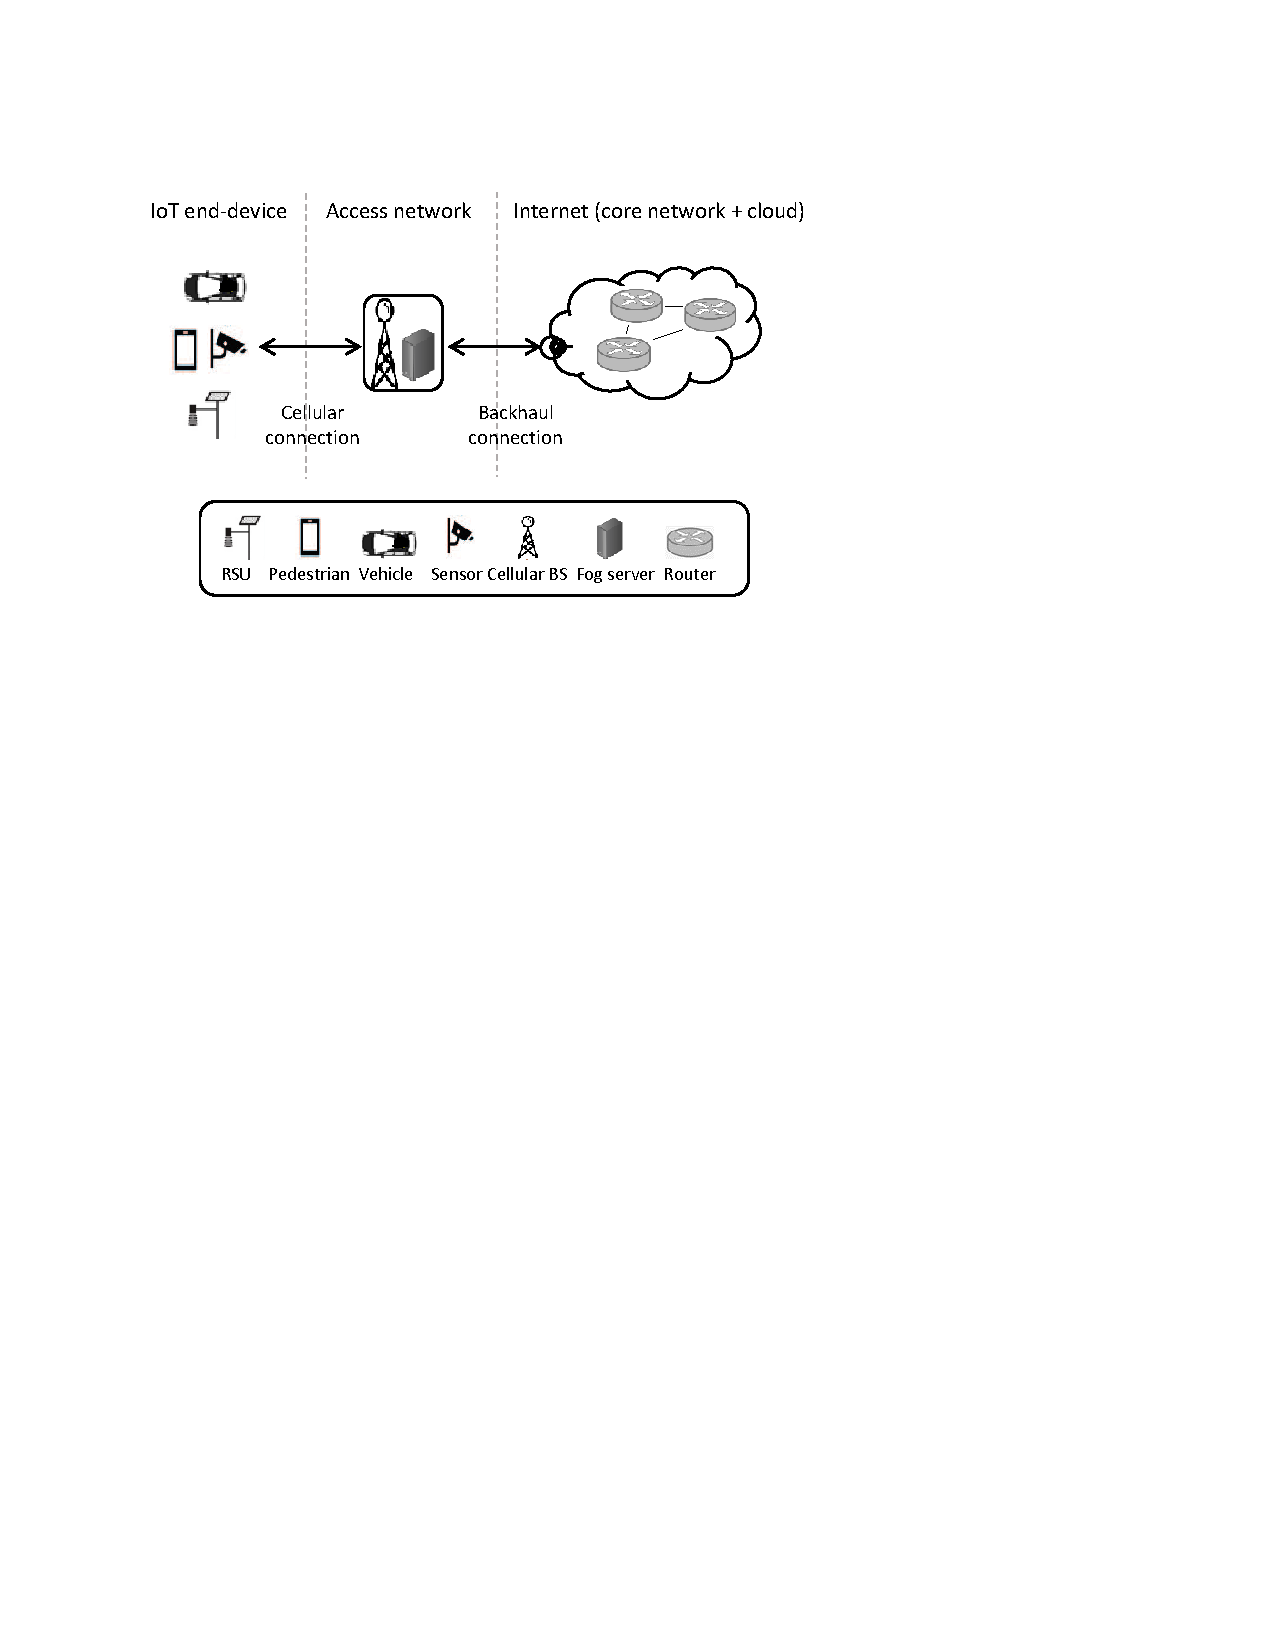
\includegraphics[clip, trim=2.5cm 17.6cm 7.8cm 3.1cm, width=\columnwidth]{figures/pdf/fig1-iot-Arch.pdf}
\caption{Overall procedure of the IoT service placement optimization}
\label{fig:system}
\end{figure}

\subsection{Problem Formulation}
\par The solution to the service placement problem is a service placement plan ($\delta$) that contains placement decisions (i.e., binary variables), which place each service either on a fog server or on a cloud center. The binary variables ${x}_{ij}$, $x_{ij'}$, and ${x}_{ik}$ denote whether service i is placed on the fog node j (the connecting node) or the fog node j' (i.e. other neighboring nodes, or the cloud node k, respectively. $\overline{x}_{ij}$ denotes the initial configuration of i on j, which indicates whether j currently hosts the service.
Also note that we consider a discrete time-slotted system model where time is divided into time slots called configuration intervals. We assume that services are always generated at the beginning of a time slot. Then each time slot becomes a decision round. Hence, we denote both time slot and decision round as $\tau$ in seconds. Table~\ref{tab:notation} lists the notations used in the problem formulation. Fig.??? We would like to draw the reader's attention to the fact that we have willingly ignored the some indexes to lighten the model (e.g., the notation $rq_{i}$ rather than $rq_{I_{i}}$).

\begin{equation}
x_{ij} = \left\{
\begin{array}{rl}
1 & \text{if  service i is hosted on fog node j}\\
\label{eq:1}\\
0 & \text{otherwise}
\end{array} \right.
\end{equation}

\begin{equation}
x_{ik} = \left\{
\begin{array}{rl}
1 & \text{if service i is hosted on cloud node k}\\
\label{eq:2}\\
0 & \text{otherwise} 
\end{array} \right.
\end{equation}
%\textcolor{red}{I have one question here: is our approach a dynamic one? Yes. According to the literature a dynamic approach is defined as follows: "To deal with the dynamic nature of Fog infrastructure and/or applications, it is required to define reactive strategies able to determine when adaptation is required, provide a transparent mechanism, and deliver the satisfying QoS. Thus, an approach is said to be dynamic if the provided placement strategy is able to deploy new services, replace or release services already deployed, in order to meet the QoS constraints and optimize a given objective (if any)."}

\tablefirsthead{%
\hline
\multicolumn{1}{|l}{Notation} &
\multicolumn{1}{l|}{Meaning} \\
\hline}
\tablehead{\hline
\multicolumn{1}{|l}{Notation} &
\multicolumn{1}{l|}{Meaning} \\
\hline}
\tabletail{%
\hline
\multicolumn{2}{|r|}{\small\sl continued on next column}\\
\hline}
\tablelasttail{\hline}
\topcaption{Mathematical Notations}\label{tab:notation}
\scriptsize
\begin{supertabular}{|p{1.3cm}p{5.8cm}|}
\hline
    C&Set of cloud nodes\\
    F&Set of fog nodes\\
    I&Set of services/vehicles\\
    $v_{i}$&Speed of vehicle i\\
    P&Set of access points in the communication network\\
    $R_{c}$&Set of core routers in the communication network\\
    $R_{e}$&Set of edge routers in the communication network\\
    S&Set of switches belonging to a cloud center\\
    $\tau$&Time interval between two instances of solving optimization
problem (in seconds)\\
\hline
    $F^{p}_{k}$&Processing capacity of cloud node k (in MIPS)\\
    $F^{m}_{k}$&Memory capacity of cloud node k (in bytes)\\
    $F^{s}_{k}$&Storage capacity of cloud node k (in bytes)\\
    $F^{e}_{k}$&Power capacity of cloud node k\\
    $F^{p}_{j}$&Processing capacity of fog node j (in MIPS)\\
    $F^{m}_{j}$&Memory capacity of fog node j\\
    $F^{s}_{j}$&Storage capacity of fog node j\\
    $F^{e}_{j}$&Power capacity of fog node j\\
	$u_{j}$ &Processing utilization of fog node j\\
	$u_{k}$ &Processing utilization of cloud node k\\
    $\mu_{j}$&Service rate of one processing unit of fog node j (in MIPS)\\
    $\mu_{k}$&Service rate of one processing unit of cloud node k (in MIPS)\\
    $n_{j}$&Number of processing units of fog node j\\
    $n_{k}$&Number of processing units of cloud node k\\
\hline    
    $P_{j}^{idle}$&Power consumption of fog node j in idle mode
(in Watts)\\
	$P_{j}^{max}$&Max power consumption of fog node j (in Watts)\\
    $P_{k}^{idle}$&Power consumption of cloud node k in idle mode
(in Watts)\\
	$P_{k}^{max}$&Max power consumption of cloud node k (in Watts)\\
	$P^{n}_{j}$&Ratio of power supplied to fog node j from renewable sources\\
	$PUE_{k}$&PUE of cloud data center k\\
	$p_{r}^{idle}$&Power consumption of router r in idle mode\\
    $e_{r}^{p}$&Dynamic energy consumption of a router to process a packet (in Joules)\\
    $e_{r}^{f}$&Dynamic energy consumption of a router to store and forward a Byte (in Joules)\\
    $p_{s}^{idle}$&Power consumption of networking element of cloud k in idle mode (in Watts)\\
    $e_{s}^{p}$&Dynamic energy consumption of switch s to process a packet (in Joules)\\
    $e^{f}_{s}$&Dynamic energy consumption of switch s to store and forward a Byte (in Joules)\\    
\hline
    $L_{i}^{p}$&CPU demand of service i (in million instruction per request)\\
    $L_{i}^{m}$&Memory demand of service i (in bytes)\\
    $L_{i}^{s}$&Storage demand of service i (in bytes)\\
    $h_{i}$&Deadline for service i\\
	$w_{ij}$&Processing and queuing delay for i served by fog node j\\
	$w_{ik}$&Processing and queuing delay for i served by cloud server k\\
\hline
	$rq_{i}$&Average size of requests of service i (in bytes)\\
    $rp_{i}$&Average size of responses of service i (in bytes)\\
    $z_{ij}$&Traffic arrival rate of service i to node j (request/second)\\
    $z_{ik}$&Traffic arrival rate of service i to node k (request/second)\\
	$z_{ijj'}$&Traffic arrival rate of service i from j to $j'$ (request/second)\\
	$z_{ijk}$&Traffic arrival rate of service i from j to k (request/second)\\
\hline
    $pd_{jj'}$&Propagation delay link $(j,j')$\\
    $rd_(jj')$&Average transmission rate of the link $(j,j')$\\
\hline
    $C_{j}^{p}$&Unit cost of processing at fog node j (per million instructions)\\
	$C_{k}^{p}$&Unit cost of processing at cloud node k (per million instructions)\\
	$C_{j}^{s}$&Unit cost of storage at fog node j (byte per second)\\
	$C_{k}^{s}$&Unit cost of storage at cloud node k (byte per second)\\
	$C_{jj'}^{c}$&Communication cost of link $(j,j')$ per unit bandwidth per sec\\    
	$C_{v}^{i}$&Cost of deadline violation per request of service (in dollar per request per \%)\\
	$C_{e}$&Cost of energy consumption per unit joul\\	
	$C_{c}$&Cost of carbon footprint\\
\hline
	$x_{ij}$&Binary decision for i on directly connected fog node j\\
    $x_{ij'}$&Binary decision for i on fog node $j'$\\
    $x_{ik}$&Binary decision for i on cloud node k\\
\hline
	$\delta$&Service placement plan\\
    $O_{\delta}^{p}$&Cost of processing for plan $\delta$\\
    $O_{\delta}^{S}$&Cost of storage for plan $\delta$\\
    $O_{\delta}^{C}$&Cost of communication for plan $\delta$\\
    $O_{\delta}^{D}$&Cost of deployment for plan $\delta$\\
    $O_{\delta}^{V}$&Cost of deadline violation for plan $\delta$\\
    $O_{\delta}^{E}$&Cost of energy consumption for plan $\delta$\\
    $O_{\delta}^{F}$&Cost of carbon footprint for plan $\delta$\\
    $\sigma_{\delta}$&Utilization variance of plan $\delta$\\
    $\omega_{\delta}$&Energy consumption variance of plan $\delta$\\
\hline
\end{supertabular}
\normalsize

\subsubsection{Application}
\par Analyst firm ABI Research \footnote{https://www.abiresearch.com/press/augmented-reality-redefine-automotive-user-interfa/} predicts that 15 million AR HUDs will ship by 2025, with 11 million to be built right into cars. In this paper, we consider passenger-facing Civil Maps'\footnote{https://medium.com/@CivilMaps/when-augmented-reality-does-its-job-well-all-want-a-self-driving-car-ba514785dbd4} augmented reality similar to 2020 Mercedes-Benz GLE\cite{abdi2015vehicle} display as our application, which requires high computation and short latency, and enables vehicles to gain a more holistic view of their current situation, assisted by the fog components. At the same time, the passengers can gain enhanced situational awareness and develop trust in the car’s competence at interpreting its surroundings.

\par In such an augmented reality application mobile devices are sending continuous flows of data to the node hosting the IoT service for processing\cite{li2017leveraging,rao2012cloud}.
We make the assumption that all the considered vehicles are equipped with an on-board camera and are capable of uploading the video/images captured by their cameras continuously to the fog and core clouds. These servers analyze each data stream and return the road condition (e.g., updated maps) to the clients. The Sense-Process-Actuate Model is used for this applications based on which data is collected by the connected sensors located at the end-devices; next, it is transmitted as data streams to the computing nodes in the higher layer (fog and/or cloud) to process and finally, the resultant commands are forwarded to the actuators\cite{azizi2019priority,gupta2017ifogsim}.

\par Processing of AR requests using nearby fog servers leads to fast distribution of critical information, i.e., obstacle detection, emergency report, collision notification, and preventing traffic jam\cite{li2018end}.
\subsection{Service placement plan}

\subsection{Local Cost}\label{subsec:localcost}
\par This section formulates the overall cost involved in executing a typical service placement plan $\delta$. This work considers the seven parameters as execution and communication costs along with penalty cost for deadline violation as a metric for QoS as follows. Other expenses can also be identified such as security safeguards, migration, etc \cite{salaht2020overview} which are not the focus of this paper. 
\begin{itemize}[noitemsep, topsep=4pt]
\item	Cost of processing in cloud and fog as $O^{P}_{\delta}$
\item	Cost of storage in cloud and fog as $O^{S}_{\delta}$
\item	Cost of container deployment as $O^{D}_{\delta}$
\item	Cost of communication as $O^{C}_{\delta}$
\item	Cost of service deadline violation as $O^{V}_{\delta}$
\item 	Cost of power consumption $O^{E}_{\delta}$
\item	Cost of carbon footprint $O^{F}_{\delta}$
\end{itemize}
\nointerlineskip

\subsubsection{Cost of processing and storage}
\par It is assumed that the processing cost in each node can be different from that of the other node. Equation (\ref{eq:3}) measures the cost of processing associated with the resource placement plan $\delta$.
\begin{equation}
\begin{aligned}
O^{P}_{\delta} = &\sum_{i=1}^{|A|}\sum_{k=1}^{|{C}|}x_{ik} \ z_{ik}  \ L_{i}^{p} \ C_{k}^{p} \ \tau + \\
&\sum_{i=1}^{|A|}\sum_{j=1}^{|{F}|}x_{ij} \ z_{ij}  \ L_{i}^{p} \ C_{j}^{p} \ \tau
\end{aligned}
\label{eq:3}
\end{equation}
\par Similar to the processing cost, the storage cost for each node is specific to that node and Equation (\ref{eq:4}) calculates this cost for the plan $\delta$.
\begin{equation}
\begin{aligned}
O^{S}_{\delta} = &\sum_{i=1}^{|A|}\sum_{k=1}^{|{C}|}x_{ik}  \ L_{i}^{s} \ C_{k}^{s} \ \tau + \\
&\sum_{i=1}^{|A|}\sum_{j=1}^{|{F}|}x_{ij} \ L_{i}^{s} \ C_{j}^{s} \ \tau
\end{aligned}
\label{eq:4}
\end{equation}

\subsubsection{Cost of service deployment and communication}
\par Cost of deployment measures the communication cost of service deployment, from cloud node to fog nodes. This paper assumes all of the services are hosted on a public cloud storage and in the case of deployment they are downloaded to the target nodes. When the demand for a deployed service is low, its host node may release that service to save more space. If a fog node accepts requests for a service not hosted locally, the service must be downloaded and deployed locally. Note that a cloud center theoretically has unlimited storage space and can host services for a long time. As a result, the communication cost for service deployment on the cloud is omitted. Equation\ref{eq:5} measures the cost of service deployment.
\begin{equation}
O_{\delta}^{D} = 
\sum_{i=1}^{|A|}\sum_{j=1}^{|{F}|}x_{ij} \ (1-\overline{x}_{ij})\ L_{i}^{s} \ C_{jk}^{c} 
\label{eq:5}\\
\end{equation}

\par Cost of communication accounts for the communication overhead related to the upload and download of data and its result known as request and response transmission. To count this cost some points must be into consideration. First, it is possible that a service is hosted on a node other than its connecting node. As a result, the required data for processing must be transferred from the connecting AP or fog node to the host fog/cloud node. Second, due to the mobility\footnote{please note that we must explain in a separate section that the vehicle traffic paths are selected in advance using EPOS so that they are known prior to the service planning(Indeed, the paths are the input of service placement algorithm).}, a vehicle may pass through several APs during the service offloading/processing. Thus, the links and networking devices connecting this vehicle to its service's host node may vary along its path. This leads to a variation in communication cost during a particular journey over one time period. Take the example of Fig.\ref{fig:comm}, the requested service for the vehicle i is supposed to be placed on the fog node $j$. At the beginning of the time interval ($t_{0}$), i is connected to j through r, while at the end of the interval ($t_{0}+\tau$), it is connected to j through both r and p. The related communication cost is calculated as follows. 
\begin{figure}[!htbp]
\centering
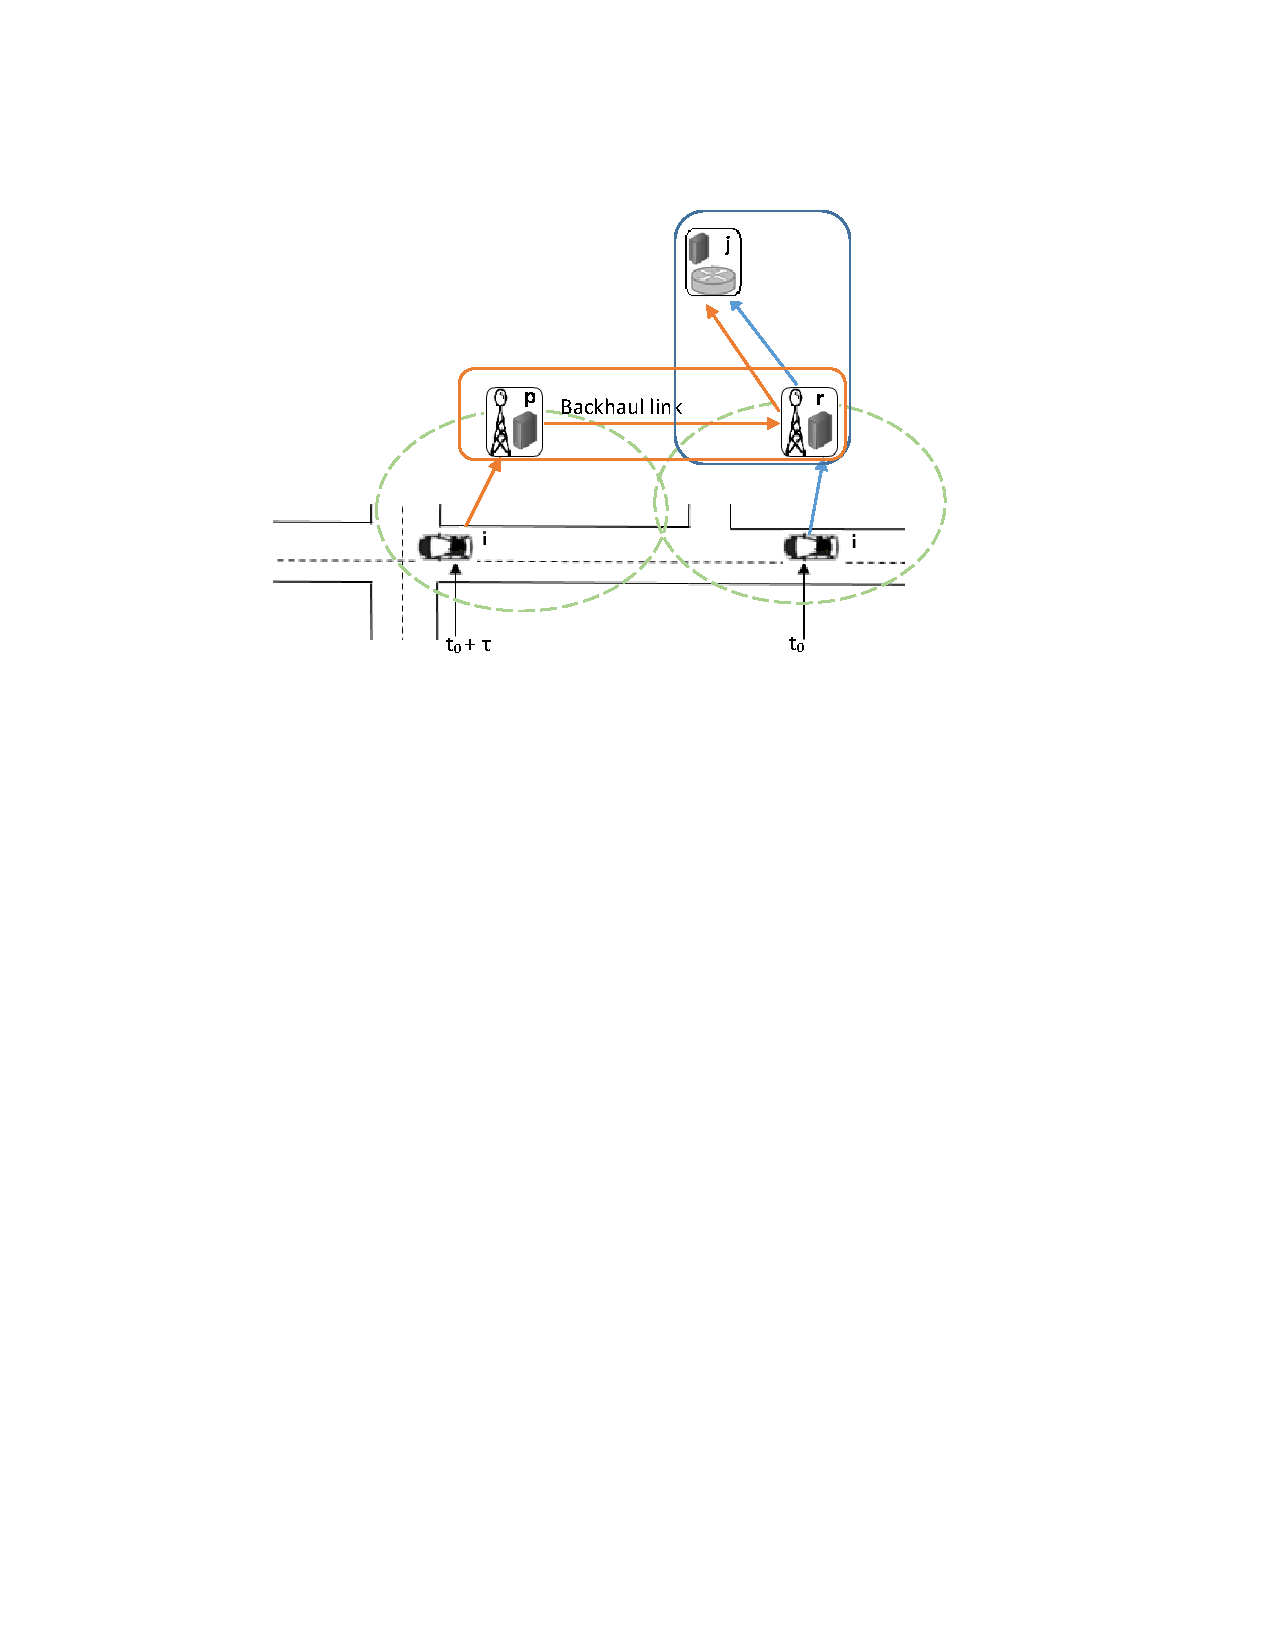
\includegraphics[clip, trim=4.2cm 15.7cm 5.2cm 3.4cm, width=\columnwidth]{figures/pdf/fig2-v2.pdf}
\caption{During one time interval ($\tau$), the connecting links and access points between the vehicle i and its host node j may change.}
\label{fig:comm}
\end{figure}
\par Let the original AP refer to the AP selected for service offloading, that is, the AP that the vehicle is currently in its coverage area and is connected to. The neighboring AP is an AP towards which (i.e. its coverage area) the vehicle moves. A relaying mechanism named handoff/handover allows a vehicle to collect the service result from the neighboring AP, if receiving the result from the original AP is not possible. In other words, the APs can communicate with each other and the service is relayed through the backhaul network and Mobile IP Protocol\cite{zhang2017mobile,li2019compound,janevski2003traffic}.
\par As a result, the communication cost consists of two parts for a time interval: 
\begin{itemize}
\item one constant component: If a vehicle is in the coverage of its target fog server, the cost of data upload/download is only the cost of the V2I (edge/core router, cloud) transmission.
\item one variable backhaul transmission component: one or more hops of backhaul transmissions and then a V2I transmission may be involved\cite{li2019compound}. 
\end{itemize}
Accordingly, Equation (\ref{eq:6}) measures the relevant communication cost.

\begin{equation}
O_{\delta}^{C} = \sum_{i=1}^{|A|} \sum_{j=1}^{|{C}\bigcup{F}|}x_{ij} \ (rq_{i}+rp_{i}) \ C_{ij}^{c} \
\label{eq:6}
\end{equation}
, where
\begin{equation}
C_{ij}^{c} = \sum_{r=1}^{|{P}\bigcup{R_{c}}\bigcup{R_{e}}|} ({\tau} z_{irj} Cirj) + \sum_{p=1}^{|P|} (z_{ipr} Cipr * {\tau}_{ip})
\label{eq:6.1}
\end{equation}
Cost $C_{irj}$ (V2I communication) is the cost of communication between a vehicle and its host server through direct V2I transmission while $C_{ipr}$ is the backhaul communication cost. The connectivity time $ {\tau}_{ip}$ estimates how long the vehicle i stays connected to an AP p (e.g., the time duration while vehicle i is in AP p coverage area). When i sends a service request to AP p with the amount of each type of data it wants to offload, its speed and data rate, as a first step, the AP calculates the connectivity time of i with further routers on the way and itself before analyzing and making offloading decision as follows:

\begin{equation}
{\tau}_{ip} = \frac{{d}_{ip}}{v_{i}}-t_{ip}-t^{w}_{ip}
\label{eq:6.1}
\end{equation}
where $d_{ip}$ is the coverage area (i.e., euclidean distance) of vehicle i with AP p while i is moving, $v_{i}$ is the speed of i, $t_{ip}$ is the registration time of i with AP p before sending service request and $t^{w}_{ip}$ is the waiting time for i to get a reply after sending request to p.
We assume...r ..p?
\subsubsection{Cost of deadline violation}
\par IoT applications like AR and VR are latency sensitive and have very rigid latency constraints in the order of tens of milliseconds\cite{la2019enabling} so that  a low latency is crucial to ensure an acceptable quality of experience. The service delay for an IoT service is defined as the time span between the moment an end-device sends its request and the moment it receives the response for that request. We need to check if the service delay ($e_{i}$) for the service i meets the delay threshold $h_{i}$ defined in SLA. Service delay includes three delay components as propagation delay, transmission delay, and waiting time (processing delay plus queuing delay)~\cite{deng2016optimal,yousefpour2019fogplan}. The binary variable $v_{ij}$ indicates the violation of deadline of service i on host node j as follows:
\begin{align}
v_{ij} & = \left\{
\begin{array}{rl}
0 & \text{if } e_{ij}<h_{i}\\
1 & \text{} otherwise
\end{array} \right.
\label{eq:8}
\end{align}
\par Delay of the service i requested by end-device i is measured as Equation (\ref{eq:9})\cite{nezami2021decentralized}. In contrast to the computation time, the communication time varies over time, because it is impacted by the fluctuation of latency between the mobile node and its processing services placed on the infrastructure. The possible causes for this fluctuation is due to the latency variation of the communication path between vehicles and their destination.

\par As discussed earlier about the Figure.\ref{fig:comm}, due to the mobility of the end-device m the connecting links between the device and its service's host node j may change over time (due to connection handoff and handover \cite{puliafito2020mobfogsim}), thereby resulting in various propagation delays and transmission rates for a particular service during one time interval. To overcome this challenge in measuring service delay, we measure those two parameters considering all of the connecting access points along the path traveled by a vehicle per time interval. The delay of a particular service is then calculated according to the estimated propagation delay and transmission rate values as Equation (\ref{eq:9}). 

\begin{equation}
\begin{aligned}
e_{i} = &x_{ij}(2pd_{irj}+\sum_{p=1}^{|P|}P_{ip}2(pd_{ipr})+\frac{rq_{i}+rp_{i}}{min(rd_{ij})}+w_{ij})
\end{aligned}
\label{eq:9}
\end{equation}
, where $rd_{ij}$ is the minimum data rate of i through the APs to j. Note that vehicles might use different devices that support different data rates. For example, it can happen that vehicle i supports higher data rate than AP p, which can cause data loss. Therefore, we take the minimum data rate between i and j as $rd_{ij}$ for smooth data transfer. Considering a set of APs located in a 2D area, $P_{ip}$ is the probability that vehicle i will be in the coverage zone of access point p during time interval $\tau$\cite{djemai2020mobility}:

\begin{equation}
P_{ip} = \frac{\tau_{ip}}{\tau} = \frac{1}{{\tau}_{ip}}*(\frac{{d}_{ip}}{v_{i}}-t_{ip}-t^{w}_{ip})
\label{eq:6.1}
\end{equation}

\par To measure the waiting time of service i hosted on node j, $w_{ij}$, we adopt multi-server M/M/c queuing model (i.e., Erlang-C\cite{gautam2012analysis})\cite{liu2019joint,zhou2018air,jia2015optimal} for the fog node j. $\zeta_{j}$ indicates the total arrival rate of instructions (in MIPS) of the incoming requests that are accepted for processing by fog node j and is calculated as follows:
\begin{equation}
\zeta_{j} = \sum_{i=1}^{|A|} L_{i}^{p} \ z_{ij} \ x_{ij}  
\label{eq:12}
\end{equation}
\par Fog node j has $n_{j}$ processing units, each with service rate $\mu_{j}$ (total processing capacity or service rate of node j is $F^{p}_{j} = n_{j} \mu_{j}$). Therefore, the waiting time for the requests of service i at fog node j is calculated as Equation (\ref{eq:13})\cite{bolch2006queueing}.

\begin{equation}
w_{ij} \triangleq  
\frac{C(n_{j},\frac{\zeta_{j}}{\mu_{j}})}{\ F^{p}_{j} f_{ij}-\zeta_{j}}+
\frac{1}{\mu_{j} \ f_{ij}}
\label{eq:13}
\end{equation}

, where $f_{ij}$ denotes the fraction of processing units that service i deployed on fog node j can obtain and is measured by Equation (\ref{eq:14}) and $\zeta_{ij}$ denotes the arrival rate of instructions (in MIPS) to fog node j for service i and measured as $\zeta_{ij} = L_{i}^{p} \ z_{ij} \ x_{ij}$.
 
\begin{equation}
f_{ij}=\frac{L_{i}^{p} \ x_{ij}}{\sum_{i=1}^{|A|} L_{i}^{p} \ x_{ij} }
\label{eq:14}
\end{equation}

According to the M/M/c queueing model, similar to the fog nodes, the computation delay for service i hosted on cloud server k with the total capacity $F^{p}_{k} = n_{k} \mu_{k}$ \footnote{For simplicity but without loss of generality, we assume that each cloud server hosts a number of homogeneous computing machines. The configurations (e.g., CPU frequency) are assumed to be equal for all machines at the same server.} is measured as follows\cite{deng2016optimal,yousefpour2019fogplan}):
%\:,\forall j\,\epsilon\,F , i\,\epsilon\,A

\begin{equation}
w_{ik} \triangleq  
\frac{C(n_{k},\frac{\zeta_{k}}{\mu_{k}})}{\ F^{p}_{k} \ f_{ik}-\zeta_{k}}+
\frac{1}{\mu_{k} \ f_{ik}}
\label{eq:15}
\end{equation}

where $f_{ik}$ denotes the fraction of processing units assigned to service i by cloud server k calculated by Equation (\ref{eq:16}) and $\zeta_{k}$ denotes the total traffic arrival rate of requests to cloud server k and is calculated by Equation (\ref{eq:17}).

\begin{equation}
f_{ik}=\frac{L_{i}^{p} \ x_{ik}}{\sum_{i=1}^{|A|} L_{i}^{p} \ x_{ik} }
\label{eq:16}
\end{equation}

\begin{equation}
\zeta_{k} = \sum_{i=1}^{|A|} L_{i}^{p} \ z_{ik} \ x_{ik}  
\label{eq:17}
\end{equation}

%delay of container deployment
%Deploy and Release Delay: One question that we need to answer is: how much delay does deploying or releasing a service incur? Is this delay negligible in practical fog networks? If deploying or releasing services fog service causes extra delay, this could have a significant impact on QoS. Nonetheless, deploying and releasing containers takes less than 50 ms [48], wheres the interval of monitoring traffic and running the FOGPLAN for deploying services in a real-world setting would be in the order of tens of seconds to minutes. In our simulations, the start-up delay of the service containers is set to 50 ms.
\par Finally, according to the QoS requirement, deadline violation should be considered with respect to the percentage of samples/requests from IoT services that their service delay exceed the delay threshold. 
Let's assume that desired quality of service for service i is denoted by $q_{i}\,\epsilon\,(0,1)$ and the percentage of delay samples from vehicles that exceed the delay threshold should be no more than $(1 - q_{i}) $\footnote{Amazon Compute SLA: https://aws.amazon.com/compute/sla}. Therefore, Equation (\ref{eq:10}) calculates the cost of deadline violation. We define $v_{ipj}$ as the percentage of requests of service i hosted on node j that do not meet the delay requirement during the time connected to the access point p. 

\begin{equation}
v_{i} = \sum_{p=1}^{P} v_{ipj} P_{ip}
\label{eq:10}\\
\end{equation}

\begin{equation}
O_{\delta}^{V} = \sum_{i=1}^{|A|}\sum_{j=1}^{|{C}\bigcup{F}|}max (0 , v_{i}-(1-q_{i})) \ z_{ij} \ C_{v}^{i} \ \tau 
\label{eq:10}\\
\end{equation}

\subsubsection{Cost of power consumption}\label{subsec:localcost-pc}
here the renewable part must be deducted
\par The huge potentials of IoT are constrained by high energy consumption, limited battery capacity, and the slow progress of battery technology\cite{zhou2021green}. The annual electricity usage of just five tech groups Amazon, Google, Microsoft, Facebook and Apple is about as much as New Zealand’s, at more than 45 terawatt-hours. A considerable portion of this consumption is due to the high amount of energy consumed by edge and cloud servers while executing the computationally intensive and time critical requests from vehicles\cite{ismail2021escove}. 
\par This paper divides energy consumption of a plan into static and dynamic parts as stated in Equation\ref{eq:18}. The static energy consumption is the energy consumption without considering any workload (i.e., resources are idle)\cite{kurpicz2016much}. The dynamic part is calculated based on the current usage of computing and networking resources by the active VMs and containers\cite{ahvar2019estimating,heinrich2017predicting,salaht2020overview}. Following parts explore those parts in more detail.
\begin{equation}
O_{\delta}^{E} = \tau * C_{e} P^{static} + P_{\delta}^{dynamic}
\label{eq:18}
\end{equation}

\makebox[4.0cm][c]{}
\parbox[c]{6.0cm}{\textbf{Static power consumption part}}
\par Static power consumption part of a fog-cloud architecture includes static (i.e., idle) power consumption of load-independent part of networking devices and fog/cloud physical servers , as stated in Equation\ref{eq:19}. For the networking part, the static power consumption corresponds to the idle power consumption of edge and core routers, access points, switches (which includes the power consumption of elements such as cooling, ventilation systems, and power supply \cite{vishwanath2014modeling}) that are employed to link the fog/cloud nodes and vehicles. 

\begin{equation}
P^{static} = P^{idle}_{network} + P^{idle}_{Fog} + P^{idle}_{cloud} 
\label{eq:19}
\end{equation}
\par For a physical machine, the static power consumption corresponds to the power consumed by the server when powered on but not running any services. Our fog servers are in the form of nano data centers that consist of one single physical machine and does not have any extra additional ICT equipment such as the intra data center network elements (i.e., switches and links)\cite{ahvar2019estimating}. Data centers have non-ICT equipment such as cooling system and their energy consumption comes from physical machines plus their networking elements. To reflect the energy consumption of non-ICT equipment, the Power Usage Effectiveness, PUE\footnote{It represents the ratio between the total facility and the IT equipment power consumption. Usually, an ideal PUE value is equal to 1.0. This indicates that the power consumed by IT equipment is same as the total facility power.} is a well-known data center energy-efficiency indicator. 
Consequently, the static power consumption of the IoT network corresponds to:

\begin{equation}
\begin{aligned}
P^{static} = &\sum_{r=1}^{|{P}\bigcup{R_{c}}\bigcup{R_{e}}|}P_{r}^{idle} +\sum_{j=1}^{|{F}|}P_{j}^{idle}\\
			&+\sum_{k=1}^{|{C}|}(P_{k}^{idle} + P_{s}^{idle})*PUE_{k}
\end{aligned}
\label{eq:20}
\end{equation}
For each resource, its static energy consumption corresponds to its idle power consumption over the considered time period $\tau$. As the idle power consumption is constant over time, multiplying it by $\tau$ gives the energy consumption over the time period $\tau$. 

\makebox[4.0cm][c]{}
\parbox[c]{6.0cm}{\textbf{Dynamic power consumption part}}
\par Dynamic power consumption of an IoT network comes from load-dependent sources of energy consumption: physical machines, routers, APs, and switches inside cloud data centers. We assume that all physical machines and network elements are always active.
\begin{equation}
P^{dynamic}_{\delta} = P^{dynamic}_{network,\delta} + P^{dynamic}_{Fog,\delta} + P^{dynamic}_{cloud,\delta}
\label{eq:21}
\end{equation}

Dynamic power consumption of physical machines depends mainly on CPU utilization and can be modeled as a linear function\cite{wiesner2021leaf,lee2012energy,beloglazov2012energy,heinrich2017predicting,azizi2019priority} as Equation (\ref{eq:22}). The parameter $(P_{j}^{max}-P_{j}^{idle})/F_{j}^{p}$ determines the incremental power consumption per unit load on fog nodes. The same assumption is valid for cloud machines.

\begin{equation}
P {j}^{dynamic} \triangleq (P_{j}^{max}-P_{j}^{idle}).u_{j} \:\:\:\: ,\forall j\,\epsilon\,F,C 
\label{eq:22}
\end{equation}
, where
\begin{equation}
u_{j}=\frac{\zeta_{j}}{F_{j}^{p}} 
\label{eq:23}
\end{equation}

\par Dynamic power consumption of an intra data center network corresponds to the dynamic power consumption of switches inside the data center. When a switch carries traffic, it consumes load-dependent power for packet processing and also for storing and forwarding the payload\cite{vishwanath2014modeling,sivaraman2011profiling}. Consequently, if the switch s inside cloud center k receives $z_{ik}$ requests during a time period $\tau$, it has to process $z_{ik}.(rq_{i}+rp_{i})$ bytes during $\tau$ as computed in Equation (\ref{eq:24}).

\begin{equation}
E^{dynamic}_{s,\delta} =  \sum_{i=1}^{|A|} \ z_{ik} \ x_{ik} (p_{s}^{p} +  p_{s}^{f} \ (rq_{i}+rp_{i}))
\label{eq:24}
\end{equation}

\par In order to compute the dynamic energy consumption of the telecommunication network that is linking physical servers with the vehicles, a network with three different types of networking devices is considered: core routers and edge routers, and APs. Similarly to the dynamic energy consumption of switches in Equation (\ref{eq:24}), the dynamic energy consumption of our network for the placement plan $\delta$ is equal to Equation (\ref{eq:25}). Please note that the energy to process a packet and the energy for storing and forwarding a byte depends on the device type since devices from different types have different energy profiles.

\begin{equation}
E^{dynamic}_{network,\delta} = \sum_{i=1}^{|A|} \sum_{r=1}^{|R_{c}\bigcup R_{e}\bigcup P|} z_{irj} \ x_{ij} (p_{r}^{p} + p_{r}^{f} \ (rq_{i}+rp_{i}))
\label{eq:25}
\end{equation}
Putting it all together, the Equation (\ref{eq:26}) shows the dynamic power consumption of fog-cloud infrastructure as a result of deploying plan $\delta$.??? formula with power energy???
\begin{equation}
\begin{aligned}
P_{\delta}^{dynamic} = &\sum_{k=1}^{|C|}(P^{dynamic}_{s} +  P^{dynamic}_{k})PUE_{k}\\
					   &+\sum_{j=1}^{|F|} P^{dynamic}_{j} + P^{dynamic}_{network,\delta}
\end{aligned}
\label{eq:26}
\end{equation}

\subsubsection{Cost of carbon footprint}
\par better to add the emission of fuel consumed by vehicles 
\par GSMA, ITU, GeSI, and SBTi set science-based emission reduction targets (SBT) at the end of February 2020, committing to helping the mobile industry achieve net-zero carbon emissions by 2050\footnote{Translating green energy into 5G success for operators, by Jiang Junmu, available at: https://www.huawei.com/br/technology-insights/publications/huawei-tech/90/green-energy-5g-success-operators, last accessed: July 2021}. 
Carbon footprint becomes a key issue for deploying server equipment. According to the Shift Project report\footnote{Impact environnemental du numérique : tendances à 5 ans et gouvernance de la 5G, https://theshiftproject.org/article/impact-environnemental-du-numerique-5g-nouvelle-etude-du-shift/}, the carbon emissions from technology infrastructure and the data servers that enable cloud computing now exceed those of pre-Covid air travel. Microsoft emitted about 16m tonnes of greenhouse gas in 2020, Google 1.5m tonnes, and Amazon 44m tonnes, according to Greenpeace, an environmental lobby group\footnote{Microsoft, Google, Amazon – Who’s the Biggest Climate Hypocrite? by Elizabeth Jardim, https://www.greenpeace.org/usa/microsoft-google-amazon-energy-oil-ai-climate-hypocrite/}.
\par This paper propose to use cost of carbon footprint as one of the local costs that each network agent consider minimizing in selecting a placement plan as its candidate one.
Equation (\ref{eq:27}) calculates the cost term due to $Co_{2}$ emission, in terms of cost of carbon footprint $C_{c}$ (USD per gram) and the average carbon emission rate R found from weighted contribution of \textbf{different fuel types} (gram per KWh)\cite{hussain2019fog}. consider:?? It is worth to note that based on the U.S. Energy Information Administration (EIA) electricity generation from clean energy source is considered carbon neutral.

\begin{equation}
O^{F}_{\delta} = \sum_{j=1}^{|F \bigcup C \bigcup {s} \bigcup R_{c} \bigcup R_{e} \bigcup P|} C_{c}*R*PUE_{j}*P{j}* \frac{\tau}{3600}
\label{eq:27}
\end{equation}

\subsubsection{Constraints}
\par Resource utilization of fog nodes and cloud servers shall not exceed their capacity, as formulated by:
\begin{equation}
\sum_{i=1}^{|A|} \ L_{i}^{s} \ x_{ij}<F_{j}^{s}\text{, and} \sum_{i=1}^{|A|} \ L_{i}^{m} \ x_{ij}<F_{j}^{m} \:,\forall j\,\epsilon\,F
\label{eq:28}
\end{equation}

\begin{equation}
\sum_{i=1}^{|A|} L_{i}^{s} \ x_{ik}<F_{k}^{s}\text{, and} \sum_{i=1}^{|A|} L_{i}^{m} \ x_{ik}<F_{k}^{m}\:,\forall k\,\epsilon\,C
\label{eq:29}
\end{equation}
In addition, stability constraints of the queues for the services on fog nodes and cloud servers imply:
\begin{equation}
\zeta_{ij}<F_{j}^{p}  f_{ij}\:,\forall j\,\epsilon\,F , i\,\epsilon\,A 
\label{eq:30}\\
\end{equation}
\begin{equation}
\zeta_{ik}<F_{k}^{p}  f_{ik} \:,\forall j\,\epsilon\,F , i\,\epsilon\,A 
\label{eq:31}\\
\end{equation}
Finally, the placement of services is constrained so that each service must be hosted on at most one computational resource. Formally,
\begin{equation}
0\leq \sum_{i=1}^{|A|}\sum_{j=1}^{|{C}\bigcup{F}|}x_{ij}\leq |A|
\label{eq:32}
\end{equation}

\subsection{Global Cost}
\par Firstly I thought of this idea: aggregating coming services on the current active nodes as far as possible and then switching off underutilized nodes that contributes to the global energy saving of the system. However, this hinders reaching the workload balance and system longevity objectives. Hence, I opted energy consumption balance and workload balance as the global objectives that are explained in the below subsections.

\subsubsection{Workload balance}
\par This work's first global objective consists in minimizing utilization variance among network servers to achieve an equitable load sharing across the network. Mainly due to vehicle mobility and the random characteristics of the wireless medium, mobile IoT networks scenario is characterized by frequent changes in network availability and traffic load. Indeed, the traffic load across the networks is time-varying\cite{bozorgchenani2021computation}. Although, utilizing fog nodes can improve resource efficiency at the edge-to-cloud networks and help the execution of delay-sensitive services. At the same time, load-balancing by avoiding bottlenecks (e.g., overloaded nodes) leads to a more reliable and flexible network. A balanced distribution of workload over the network ensures the high availability of nodes to reliably forward requests to appropriate nodes~\cite{khattak2019utilization}, which reduces the probability of late response to emergencies\cite{khattak2019utilization,rahmani2015smart,gia2019exploiting}. 
\par Network nodes have different capacities, and the workload allocated to them must not exceed this capacity. Thus, the workload-to-capacity proportion is applied to formulate the utilization of the nodes. Equation~(\ref{eq:33}) shows how balanced the workload distribution (in terms of processing power) is among all nodes measured with the variance: (we might consider memory too???)
\begin{equation}
\sigma_{\delta}=\frac{1}{|F|+|C|}
\sum_{j=1}^{|{C}\bigcup{F}|}(\frac{\zeta_{j}}{F_{j}^{p}}-\overline{\frac{\zeta_{j}}{F_{j}^{P}}})^{2}
\label{eq:33}\\
\end{equation}

\subsubsection{Power consumption balance}
\par Not only from the climate change and green IoT points of view but also for the performance, service continuity and lifetime of the IoT network energy efficient resource allocation is urgent. As investigated in previous subsection~\ref{subsec:localcost-pc}, the energy consumption encompasses mostly two parts: energy consumption in the communication network and the server side. With the resource constraints and ever-increasing service requests, this paper investigate the energy consumption balance among the edge-to-cloud server nodes which is crucial and desirable to consider\cite{deng2016optimal,hassan2020priority}.
With respect to the power model discussed already, Equation~(\ref{eq:34}) shows how balanced the energy consumption is among all nodes.
\begin{equation}
\omega_{\delta}=\frac{1}{|F|+|C|}
\sum_{j=1}^{|{C}\bigcup{F}|}(\frac{P_{j}}{F^{e}_{j}}-\overline{\frac{P_{j}}{F^{e}_{j}}})^{2}
\label{eq:34}\\
\end{equation}
, where
\begin{equation}
\begin{aligned}
P_{j} = &P {j}^{static} + P {j}^{dynamic}
\end{aligned}
\label{eq:35}
\end{equation}

\subsubsection{Renewable energy consumption}
\par According to the report of International Energy Agency (IEA), generating capacity from renewable energy sources of the world will reach 8500 GW by 2050. This research concern is not only reducing energy consumption but also promoting renewable energy with incentives. Energy harvesting from renewable energy resources, such as wind and solar power is a promising field in increasing the efficiency and lifetime of IoT network and making network more sustainable from the environmental point of view\cite{lee2015powering}.
\par Li \textit{et al.}\cite{li2018enabling} implemented a prototype system by using microgrid (solar-wind hybrid energy system) and edge computing devices and demonstrate that renewable energy can fully support the reliable running of edge devices during most (94.8\%) of the test period. In 2019, Jeff Bezos unveiled a new corporate “Climate Pledge” with which, Amazon finally set a deadline to reach 100\% renewable energy and net zero carbon by 2040\footnote{https://www.greenpeace.org/usa/microsoft-google-amazon-energy-oil-ai-climate-hypocrite/}. 

\par It is assumed that fog and cloud nodes and networking devices are partly powered by clean energy and use energy storage devices\cite{ghiassi2014toward} to store the renewable energy to increase their usage of it. We suggest that nodes with a larger share of clean energy have a higher priority in service deployment. To this end, Equation (\ref{eq:27-1}) minimizes the squared Euclidean distance of network nodes' utilization from a target incentive vector formed by nodes' ratio of energy supplied from renewable sources (after scalarization). 
\begin{equation}
Min \sqrt{\frac{\sum_{j=1}^{|F \bigcup C|}(u_{j}-P^{n}_{j})^2}{|C|+|F|}}
\label{eq:27-1}
\end{equation}

\section{Mobility-aware Service Placement on the Edge }

\subsection{Plan generation}
\par This section illustrates how agents can locally and autonomously generate service placement plans for requested
IoT services. Agents prefer to minimize the execution cost of their received services, which concerns the mentioned local cost. Each agent, upon receiving IoT requests, locally generates a certain number of assigning/mapping ``requests to
resources'' called possible service placement plan, concerning the local cost. 
Possible plans are the agents' options, that encode selected hosts in the form of a binary vector, and resource utilization in the form of a vector with real values.
\par Every vehicle submits its service request to the access point which is accessible from the vehicle.
Each fog/cloud server is equipped with a software agent that autonomously generates a predefined number of assignments determining which received service is deployed on which host in the neighborhood of the agent. In other word, the access point's edge servers select the servers where their received requests' constraints are satisfied and calculate the requests' execution cost on each of the selected servers. Then agents, cooperatively, select an assignment such that their combination minimizes cost in terms of both mentioned local and global objectives.
Finally, the edge servers offload requests to the selected host for execution and this procedure repeats for coming requests. It is worth mentioning that individual fog nodes are only utilized up to 85\% capacity for the service deployment, and the rest of their capacity is reserved for maintenance.
%At the beginning of time interval (T0, T0+Δt), local cost is calculated to decide on the placement of requested services for vehicles. Firstly, access points (service hosts or fog nodes) are selected randomly, and then, the local cost of execution on those access points is calculated. To measure this cost two above mentioned components are estimated.
%1. Take the example of figure 1. We know the initial position of each vehicles and the last one (or its direction and speed) for each time interval. At each interval (Δt), service response time depends on the distance (as one factor) between source and destination nodes. Since the vehicles in our network are mobile, one service may experience a deadline violation at one point (T0, distance = D1) while not at another (T0+Δt, distance = D2), during the same time interval. I am not sure that at which point should I calculate this parameter to have a better estimation for this cost.

\par Figure.\ref{fig:go} presents a macro view of our proposed work aimed at optimizing IoT service placement over the edge-to-cloud network as a result of traffic load balance over the roads.

\begin{figure}[!htbp]
\centering
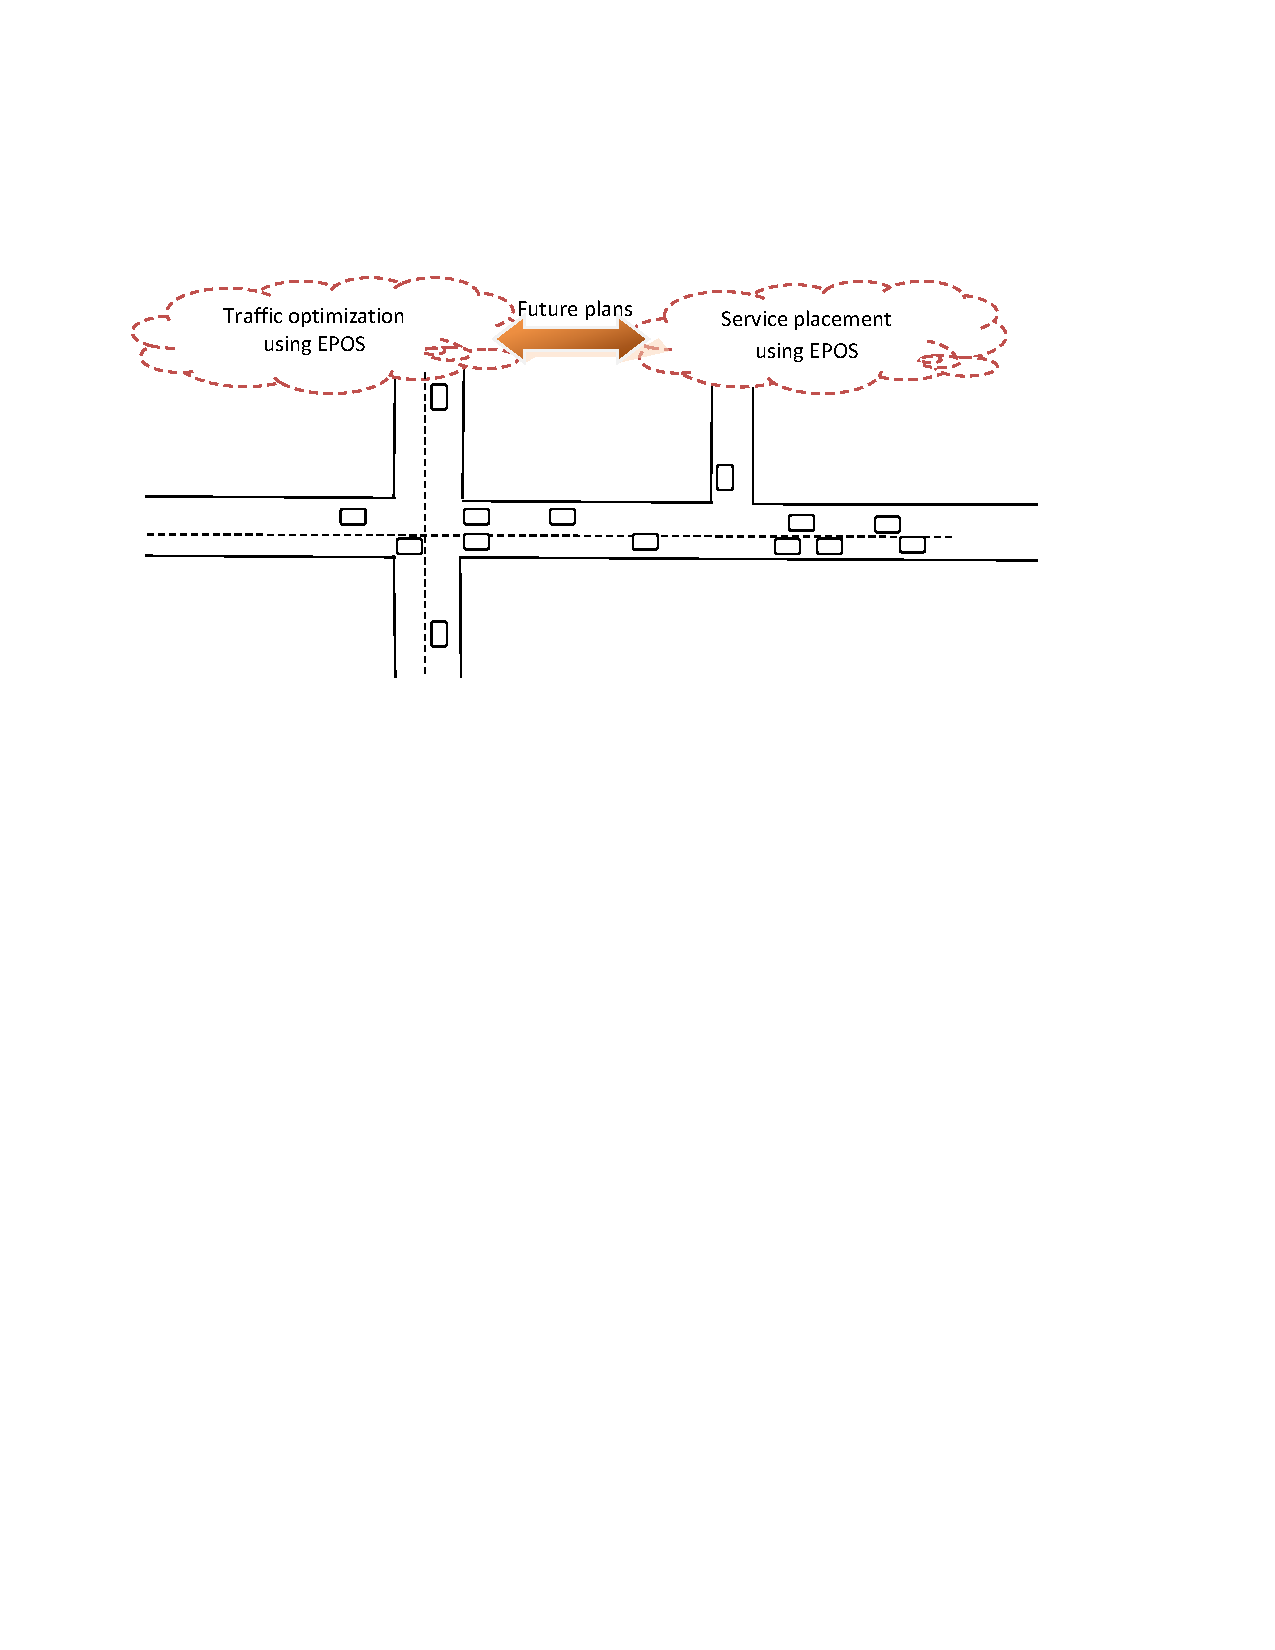
\includegraphics[clip, trim=2.1cm 17.8cm 4.2cm 4.1cm, width=\columnwidth]{figures/pdf/Macro-view.pdf}
\caption{Jointly optimizing IoT service placement and traffic load using EPOS}
\label{fig:go}
\end{figure}

\begin{figure}[!htbp]
\centering
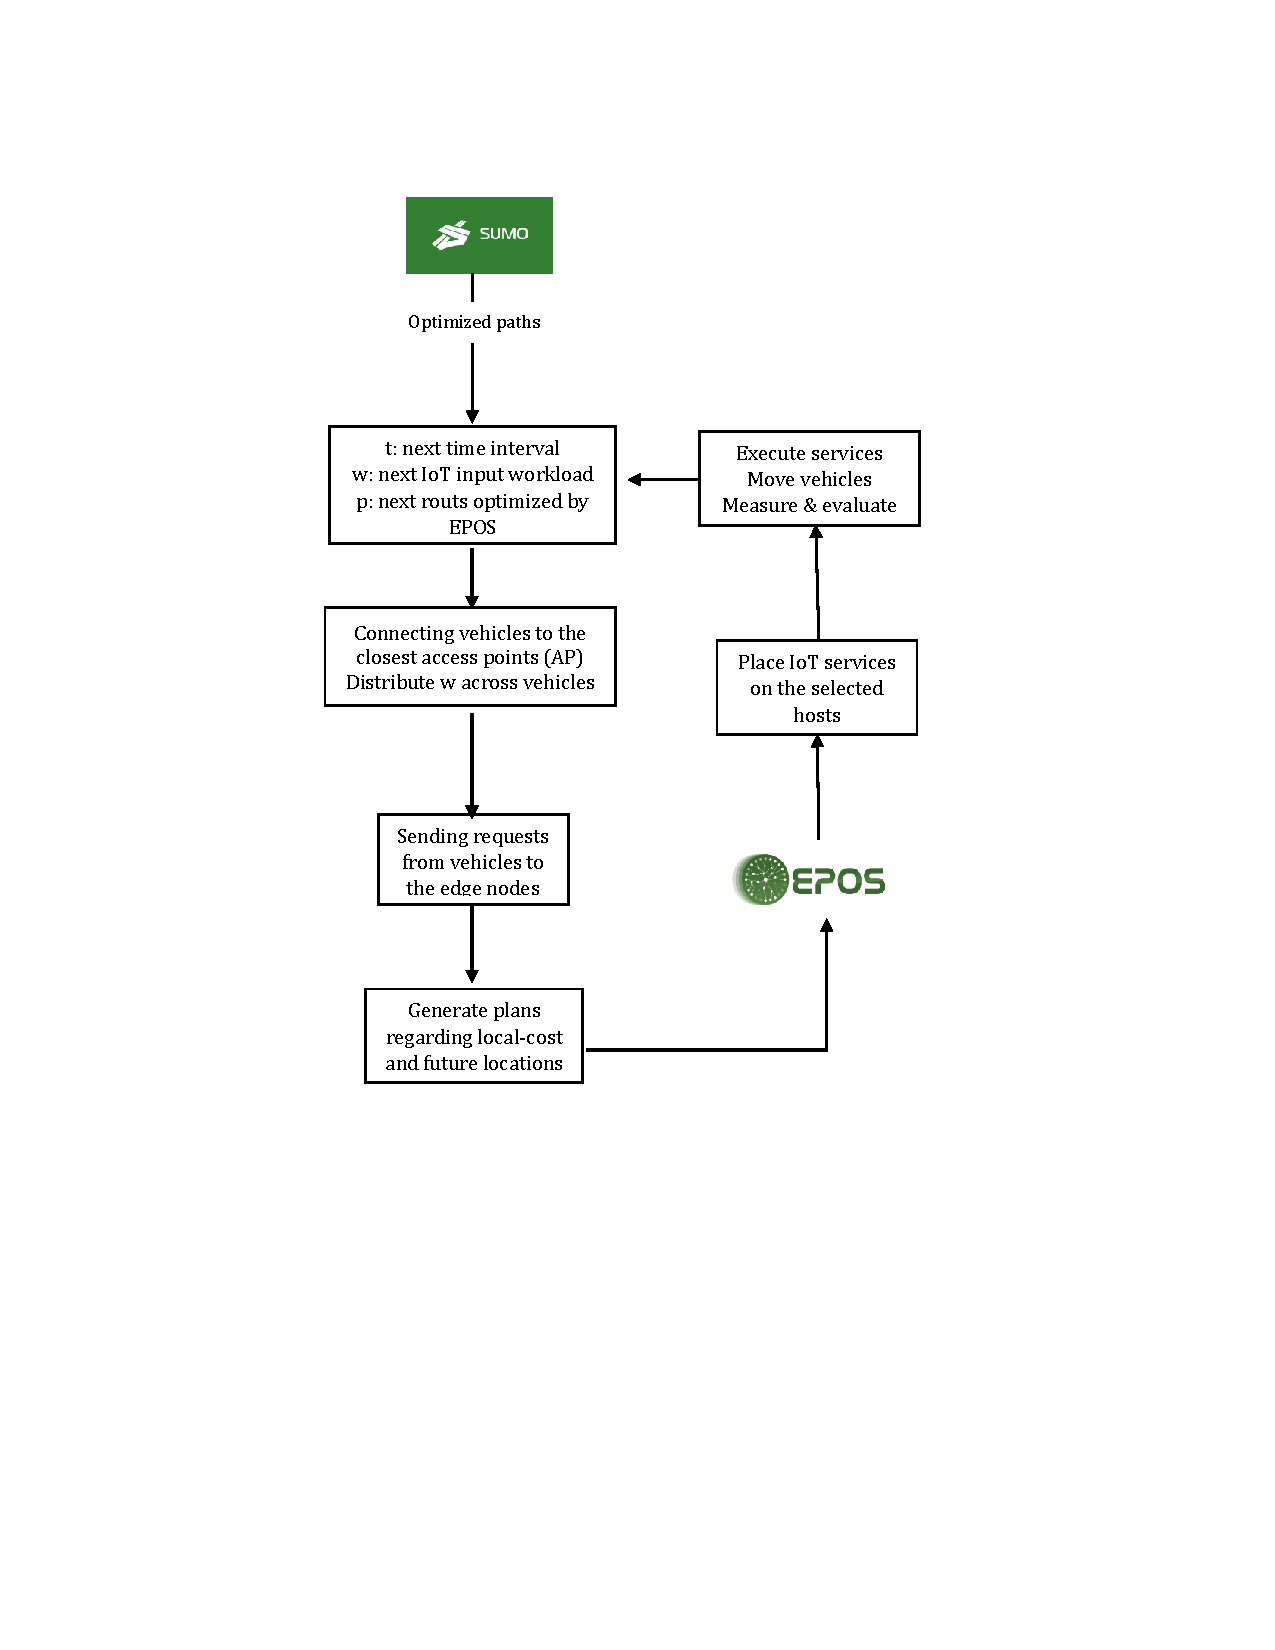
\includegraphics[clip, trim=4.5cm 9.6cm 5.6cm 3.5cm, width=\columnwidth, height=9cm]{figures/pdf/Workflow.pdf}
\caption{Overall procedure of the IoT service placement optimization}
\label{fig:workflow}
\end{figure}

\subsection{Plan selection}

\section{Evaluation}
\par To evaluate the proposed mechanism four scenarios are evaluated in this paper: 
\begin{itemize}[noitemsep, topsep=4pt]
\item Optimized service placement with basic mobility routes and optimized ones by EPOS.
\item Baseline service placement with basic mobility routes and optimized ones by EPOS.
\end{itemize}

As the basic service placement we can consider First-Fit\cite{brent1989efficient,skarlat2017} or Edge-ward\cite{gupta2017ifogsim} service placement approaches. Please let me know your opinion in this case.
\emph{First Fit}~\cite{brent1989efficient,skarlat2017}: In this approach, each node traces the latency of the communication link between itself and other nodes and sorts the list of its direct neighbor nodes. Then, upon the receipt of each request, the list is checked, and if any node in the list meets the request requirements, it is sent to that node. Otherwise, the request is propagated to the cloud.
\emph{Edge-ward}\cite{gupta2017ifogsim} is based on a First Come-First Served (FCFS) strategy it represents a placement strategy focused on the edge only.  If the edge devices does not have available computational capacity, then the algorithm searches for a fog node with capacity at the top layer of the network topology hierarchy. Edge-ward strategy iterates on fog nodes towards cloud and tries to place services on leaf-to-root paths in the physical network topology.

\subsection{Simulation setting}
\par In addition to the vehicles there are five elements in our network: cloud center, fog servers, core and edge routers, and access points.  
In the body of research on fog computing, a fog node is any computing or networking resource on the path between a data source and the center of the cloud, e.g., smart phones, routers\cite{hernandez2017implementing,shi2016edge,gupta2017ifogsim}. Also, according to European Telecommunications Standards Institute (ETSI)\cite{hu2015mobile}, edge/fog servers can be deployed at multiple locations, such as the LTE macro base station sites and aggregation points (which may also be at the edge of the core network).
\par We assume that a client connects to one fixed access point to join the network\cite{mayer2017emufog}. In addition, each network edge/backbone router is equipped with computing and storage capabilities as a fog server. The fog nodes are linked to the access points through edge routers while the cloud is reached through core routers\cite{li2018end}. 
\par Four sets of experiments are conducted within Munich, Germany. An area of 1.5 ${km}^{2}$ is selected as our test area. Each edge router is also equipped with a cell site so that takes the part of an access point/gateway for the vehicles in its vicinity to connect them to the network with the coverage range of approximately 1/2??? mile (0.80 km). The experiments are conducted on the world's largest Open Database of Cell Towers OpenCellID\footnote{https://opencellid.org} dataset. This widely-used dataset contains the locations of real-world cellular base stations. There are a total of 162 LTE base stations located within this area with a coverage radius larger than 1000m, comparable to macrocell. We plot these base stations on the map, as shown in Fig.\ref{fig:APs}. 

\par The number of core routers for our test city is extracted using Macroscopic Internet Topology Caida dataset\footnote{Macroscopic Internet Topology Caida dataset, available at: https://www.caida.org/data/internet-topology-data-kit/release-2019-04.xml} and EmuFog emulator\cite{mayer2017emufog}. Results show that there are 154 backbone routers in the city Munich. Due to Internet’s physical structure concerns, the exact location of the routers located in a city is not available publicly. However, based on the literature, in economically homogeneous regions, router density shows a strong superlinear relationship to population density\cite{canbaz2017comparative,lakhina2003geographic}. As a result, we consider one core router and one cloud center in the distance of 10 hop of our city nodes. 

\begin{figure}[!htbp]
\centering
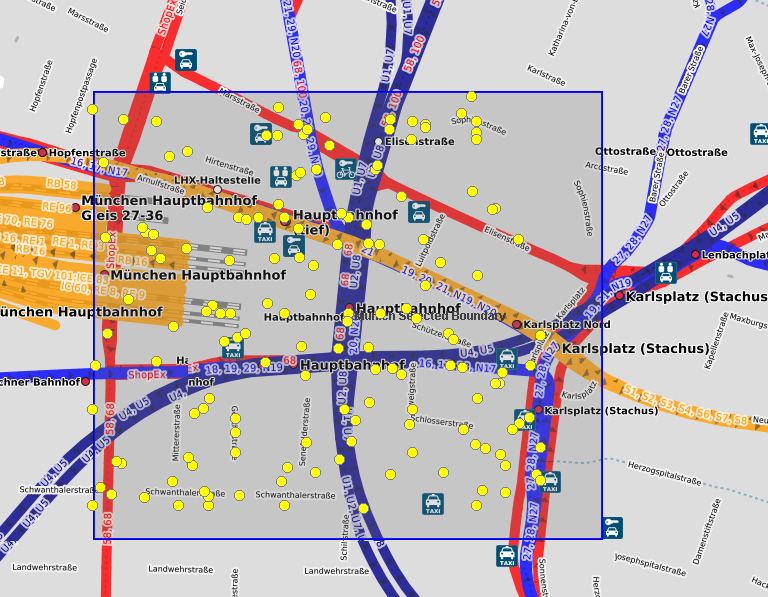
\includegraphics[clip, trim=0cm 0cm 0cm 0cm, width=\columnwidth]{figures/pdf/fig3-sim-1.4km2-bs1.PNG}
\caption{a portion of Munich city with 162 cellular base stations shown using yellow markers}
\label{fig:APs}
\end{figure}

\par Similar to Ahvar \textit{et al.}\cite{ahvar2019estimating} we assume a data center with central control that requires one switch. For the switch inside Data Center, we consider a 16-ports switch: Cisco WS-C6503 switch equipped with one 16-port WS-X6516-GE-TX line card. It consumes around 280 Watts according to the Cisco Power Calculator \footnote{Cisco’s power consumption calculator. [Online]. Available:http://tools.cisco.com/cpc}. Real measurements in\cite{vishwanath2014modeling,sivaraman2011profiling} show that there is not a visible difference between $E^{p}_r$ for various routers. Therefore, we simply assume the same value of 1300 nJ/pkt for all types of routers and switches. Similarly, we consider $E^{sf}_r=14$ nJ/Byte for all network elements. Fog server characteristics are listed in Table.\ref{tab:1}.

\begin{table}[tb]
\setlength\tabcolsep{0pt}
\scriptsize\centering
\caption {Edge servers characteristics and power consumption~\cite{gupta2017ifogsim,taneja2017resource}}\label{tab:1}
\smallskip
%\begin{tabular*}{\columnwidth}{@{\extracolsep{\fill}}lr}
\begin{tabular*}{7cm}{|p{2cm}p{2cm}p{1.5cm}p{1.5cm}|}
\hline
Processing power (MIPS)&Memory(MB)&$P^{max}_{j}$(watt)&$P^{min}_{j}$(watt)\\
\hline
    300&256&88.7&82.7\\
    1400&2048&107&83.2\\
   	1600&1024&87.5&82.4\\
   	3000&4096&107.3&83.4\\
   	10000&10240&412&333\\
\hline
\end{tabular*}
\end{table}

\begin{table}[tb]
\setlength\tabcolsep{0pt}
\scriptsize\centering
\caption {Networking equipment and servers power consumption using Cisco hardware power consumption determined with the Cisco Power Calculator~\cite{wiesner2021leaf}}\label{tab:2}
\smallskip
%\begin{tabular*}{\columnwidth}{@{\extracolsep{\fill}}lr}
\begin{tabular*}{8cm}{|p{4cm}p{2cm}p{2cm}|}
\hline
Device type&$P^{max}_{j}$(nj/bit)&$P^{min}_{j}$\\
\hline
    4G LTE access network&6200&20500\\
    Edge router (Cisco ASR 9010)&5.9&5.9\\
   	Core routers (5x Cisco CRS-3)&13.5&13.5\\
   	Cloud switche (2x Cisco Nexus 9500)&0.4&0.4\\
   	Cloud node&700$\mu$.W/mips&0\\
   	Fog node(maxload=400000mips)&350$\mu$w/mips&100w\\
\hline
\end{tabular*}
\end{table}

\begin{table}[thb]
\setlength\tabcolsep{0pt}
\scriptsize\centering
\caption {Networking equipment and servers power consumption~\cite{jalali2016fog}}\label{tab:4}
\smallskip
%\begin{tabular*}{\columnwidth}{@{\extracolsep{\fill}}lr}
\begin{tabular*}{7cm}{|p{3cm}p{2cm}p{2cm}|}
\hline
param&Edge router&Core router\\
\hline
   Idle consumption&4.09&11.07\\
   Max consumption&4.55watt&12.3watt\\
   Energy&37nj/bit&12nj/bit\\
\hline
\end{tabular*}
\end{table}
\par For a fog server, a raspberry Pi processor is used. We assume 2 instructions per cycle for the raspberry Pi processor, with 4 cores of speed = 1200 MHz\cite{bekaroo2016power}. Other values are listed in Table.~\ref{tab:5}\footnote{R. Pi. (Sep 2021). Raspberry Pi 3 Model B. Available:https://www.raspberrypi.org/documentation/, Intel. (Sep 2021). Intel® Xeon® Processor E5-2680 v2. Available:https://ark.intel.com/content/www/us/en/ ark/products/75277/intelxeon-processor-e5-2680-v2-25m-cache-2-80-ghz.html, Espressif. (Sep 2021). ESP8266EX Datasheet. Available: https://www.espressif.com/en/support/download/documents, R.Pi...??}.

\begin{table}[!htbp]
\setlength\tabcolsep{0pt}
\scriptsize\centering
\caption {Mathematical Notations}\label{tab:5}
\smallskip
\begin{tabular*}{8.0cm}{|p{3.5cm}p{1.2cm}p{1.3cm}p{2cm}|}
\hline
description&idle power&busy power&k\\
\hline
    edge node-rasberry pi 2 instructions/cycle x 4 cores.1200 MHz = 9600 MIPS&2w&12.5w&(12.5-2) /9600 = 0.0011 W/MIPS\\
    Access Point&5.5w&25w&0\\
	onu&13.5w&15w&0\\
	cloud 4 instructions/cycle x 10 cores x 2.8 GHz =112000 MIPS&57w&115w&(115--57)/112000= 0.000518 W/MIPS\\
\hline
\end{tabular*}
\end{table}

\par With respect to the current default configuration for Amazon EC2 Instance Types:
(i) The storage capacity of the fog nodes is assumed to be more than 25 GB, to host at most 50 services of the maximum size. The storage capacity of the cloud servers is 10 times that of the fog nodes. (ii) Fog nodes are assumed to have 4 processing units whereas cloud servers assumed to have 8. The capacity of the links between data generators and fog nodes is considered to be 1 Gbps whereas the inter-fog communication link capacity is taken as 10 Gbps\cite{hussain2019fog,yousefpour2019fogplan}.

\par The propagation delay can be estimated by halving the round-trip time of small packets; and as evaluated in \cite{yousefpour2018reducing}; it is assumed to be U(1; 2) ms between the IoT nodes and the fog nodes, and U(15; 35) ms between the fog nodes and the cloud servers. 
%The transmission medium
%between the IoT nodes and the fog nodes is assumed to be
%either (50\% chance for each case) one hop WiFi, or WiFi and
%a 1 Gbps Ethernet link. The fog nodes and the cloud servers
%are assumed to be 6-10 hops apart, while their communication
%path consists of 10 Gbps (arbitrary) and 100 Gbps (up to 2)
%links. The transmission rate of the link between the FSC and
%the fog nodes is assumed to be 10 Gbps.
%4) QoS parameters: The level of quality

\par We consider a PUE value of 1.2 for data center. As a comparison, Google currently exhibits an average PUE of 1.10 on its data centers\footnote{Google Data Centers Efficiency, accessed in August 2021, [online] https://www.google.com/about/datacenters/efficiency/}. The cost corresponding to consumed power is uniformly distributed between USD 30/MWh and USD \$70/MWh \cite{wu2015cloud}. For cost analysis, the cost of a 1 Gbps and 10 Gbps gateway router port is kept at USD 50 each per year while cost of server is USD 4000 per year \cite{wu2015cloud}. Upload tariff is USD 12 per byte while storage cost is kept in the range of USD 0.45–0.55 per hour\cite{hussain2019fog}. The penalty corresponding to CO2 emission is USD 51 per tons of CO2 emitted\footnote{https://ember-climate.org/data/carbon-price-viewer/ and https://www.statista.com/statistics/483590/prices-of-implemented-carbon-pricing-instruments-worldwide-by-select-country/, https://www.scientificamerican.com/article/cost-of-carbon-pollution-pegged-at-51-a-ton/}.
\par According to the U.S. Energy Information Administration (EIA) report in 2019, average carbon emission rate (R) equals 0.92 pounds of CO2 emissions per kWh. Price of renewable energy sources is (\$/kWh) 200\cite{li2017balancing}.

%ICAP’s “Emissions Trading Worldwide: Status Report 2021” shows
%In 2019 many governments began the push for carbon neutrality with national targets and new policy strategies. The International Carbon Action Partnership's (ICAP) “Emissions Trading Worldwide: Status Report 2020” finds that 
%in europe: The carbon price signal remained strong, levelling at an average of almost EUR 25 (USD 28.55) per tonne CO2e. 
%\footnote{Source: ICAP. (2021). Emissions Trading Worldwide: Status Report 2021. Berlin: International Carbon Action Partnership, 2021, https://icapcarbonaction.com/en/?option=com_attach&task=download&id=723}

%The economic downturn caused by COVID-19 has seen a decline in allowances prices in
%various ETSs. This is to be expected with allowances prices being a function of demand and supply.
%The EU ETS allowance prices decreased in the first quarter of 2020 to \euro17/tCO2e (US$19/tCO2e)
%compared to around €25/tCO2e (US$27/tCO2e) over 2019. Similarly, allowance prices in the
%California-Québec carbon market dropped below the 2020 auction reserve price of US$17/tCO2e.
%The COVID-19 pandemic has also affected prices in various carbon taxes. Newfoundland and
%Labrador had planned to raise its carbon tax to CAN$30/tCO2e (US$21/tCO2e) on April 1, 2020, but
%this has been delayed until further notice due to impacts of COVID-19. Similarly, British Columbia
%froze its carbon tax rate at CAN$40/tCO2e (US$28/tCO2e), postponing its decision to increase it
%to CAN$45/tCO2e (US$40/tCO2e) until further notice. It also increased and expanded the British
%Columbia climate action tax credit to provide income support for its residents.
%\footnote{: World Bank.“State and Trends of Carbon Pricing 2020” (May), World Bank, Washington, DC. Doi: 10.1596/978-1-4648-1586-7, 2020, https://www.ieta.org/resources/Conferences_Events/2020/Carbon%20Market%20Virtual%20Series/WB%20State%20and%20Trends%202020_Full%20report.pdf}

\subsection{Workload} 
\begin{figure}[!htbp]
\centering
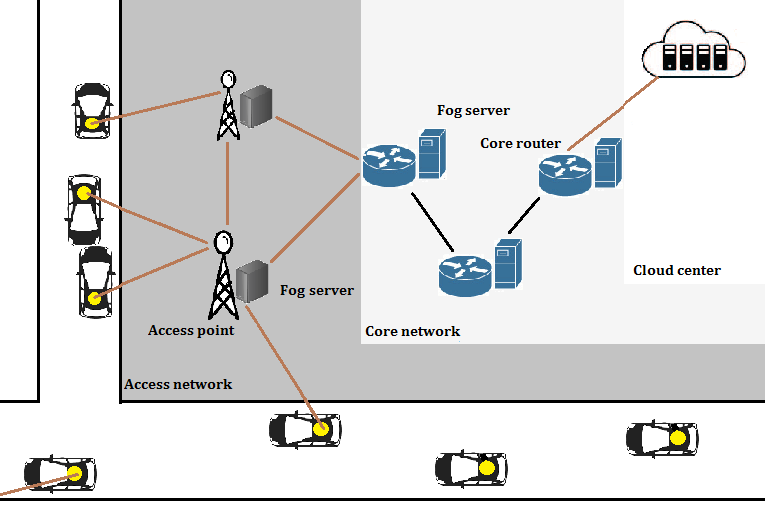
\includegraphics[clip, trim=0.0cm 0.2cm 0.5cm 0.3cm, width=\columnwidth]{figures/candid-arch.png}
\caption{Edge–cloud system model for vehicular networks.}
\label{fig:app}
\end{figure}
\par We study the road traffic distribution pattern in the city area of Munich. We collect the traffic volume ??? that fall into this area according to ????.
\par As the input workload we use MAWI (Measurement and Analysis on the WIDE Internet) traffic repository\footnote{MAWI Working Group Traffic Archive, available at: http://mawi.wide.ad.jp/mawi/}. The MAWI archive is collected from the WIDE Internet backbone that connects Japanese universities and research institutes to the Internet.
Figure.\ref{fig:traffic} shows the non-normalized incoming traffic to the fog nodes used in our evaluation. 

\begin{figure}
		\centering
		\begin{subfigure}{\columnwidth}
			\centering
			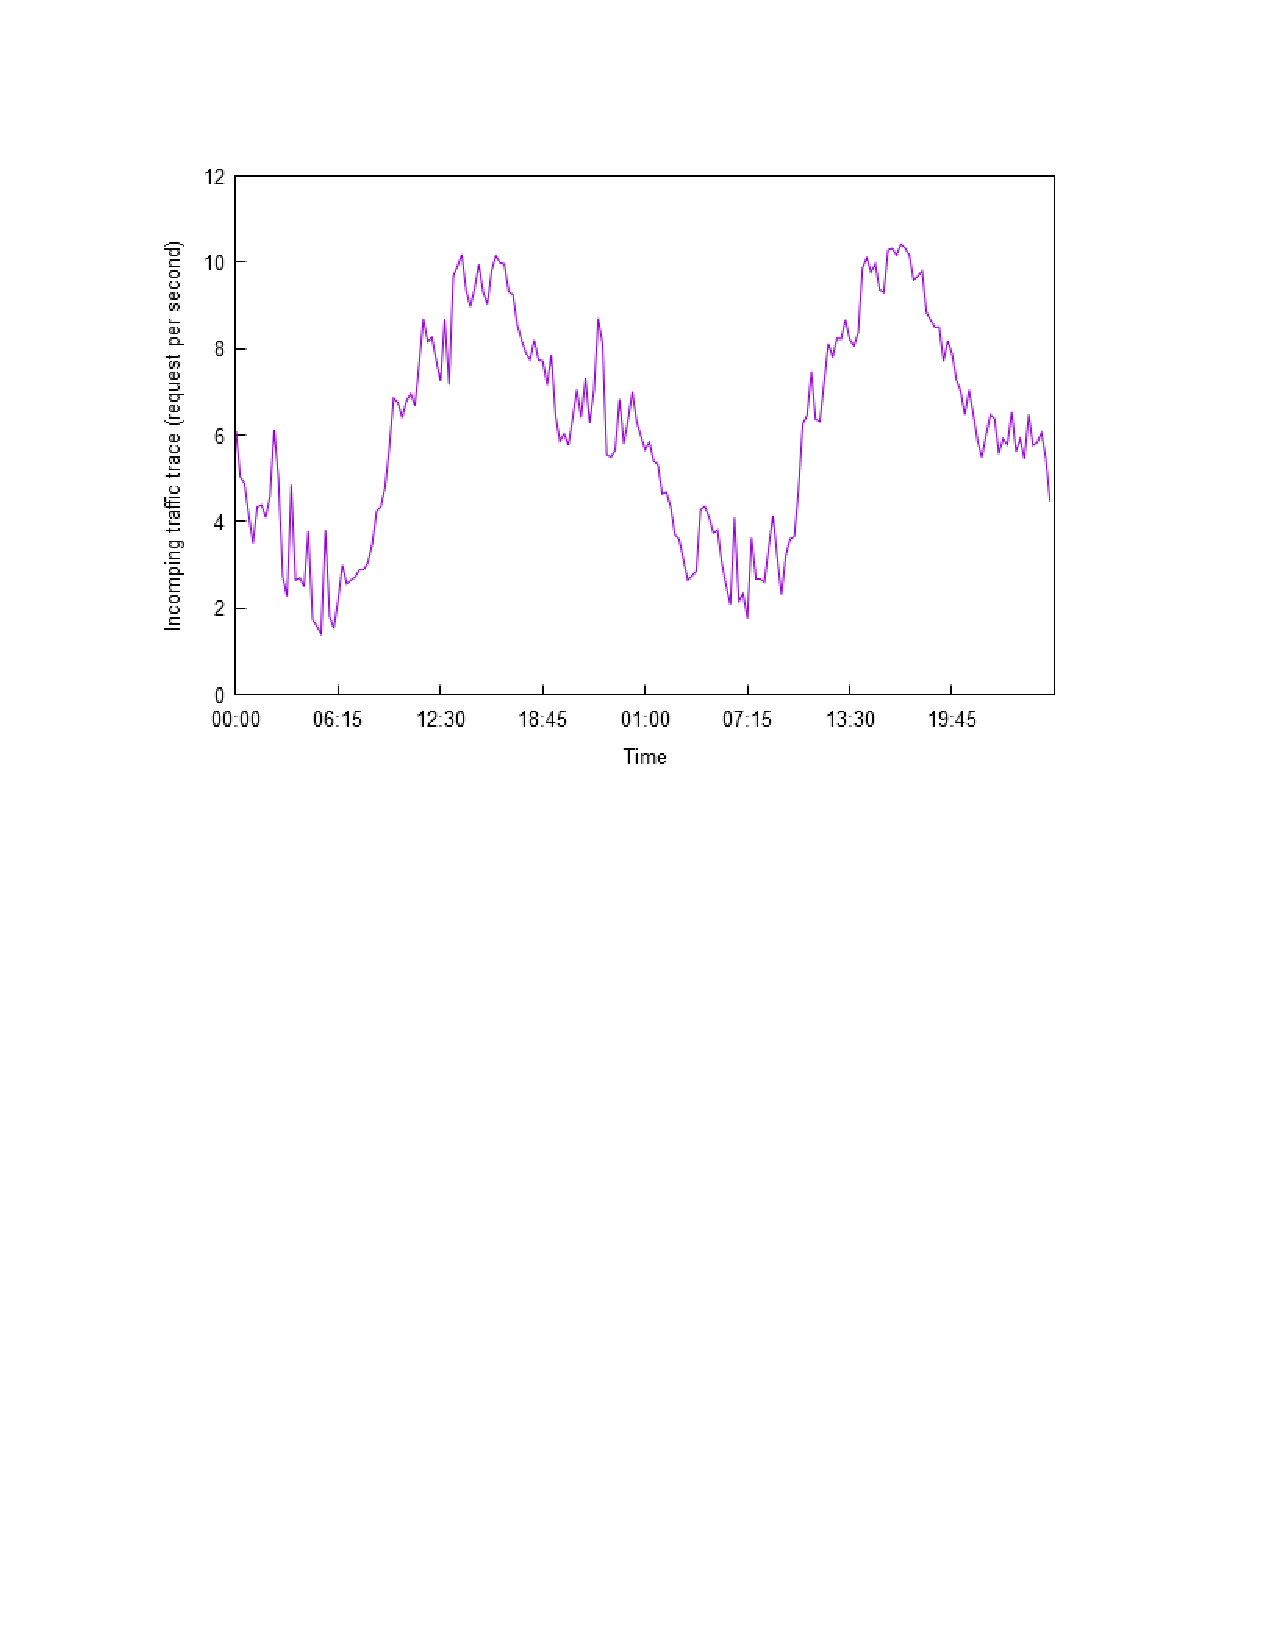
\includegraphics[clip, trim=2.5cm 15cm 3.6cm 2.5cm, width=\columnwidth]{figures/pdf/traffic-1.pdf}
			\caption{48 hours of MAWI trace data of 2017/04/12-13}
		\end{subfigure}
		\begin{subfigure}{\columnwidth}
			\centering
			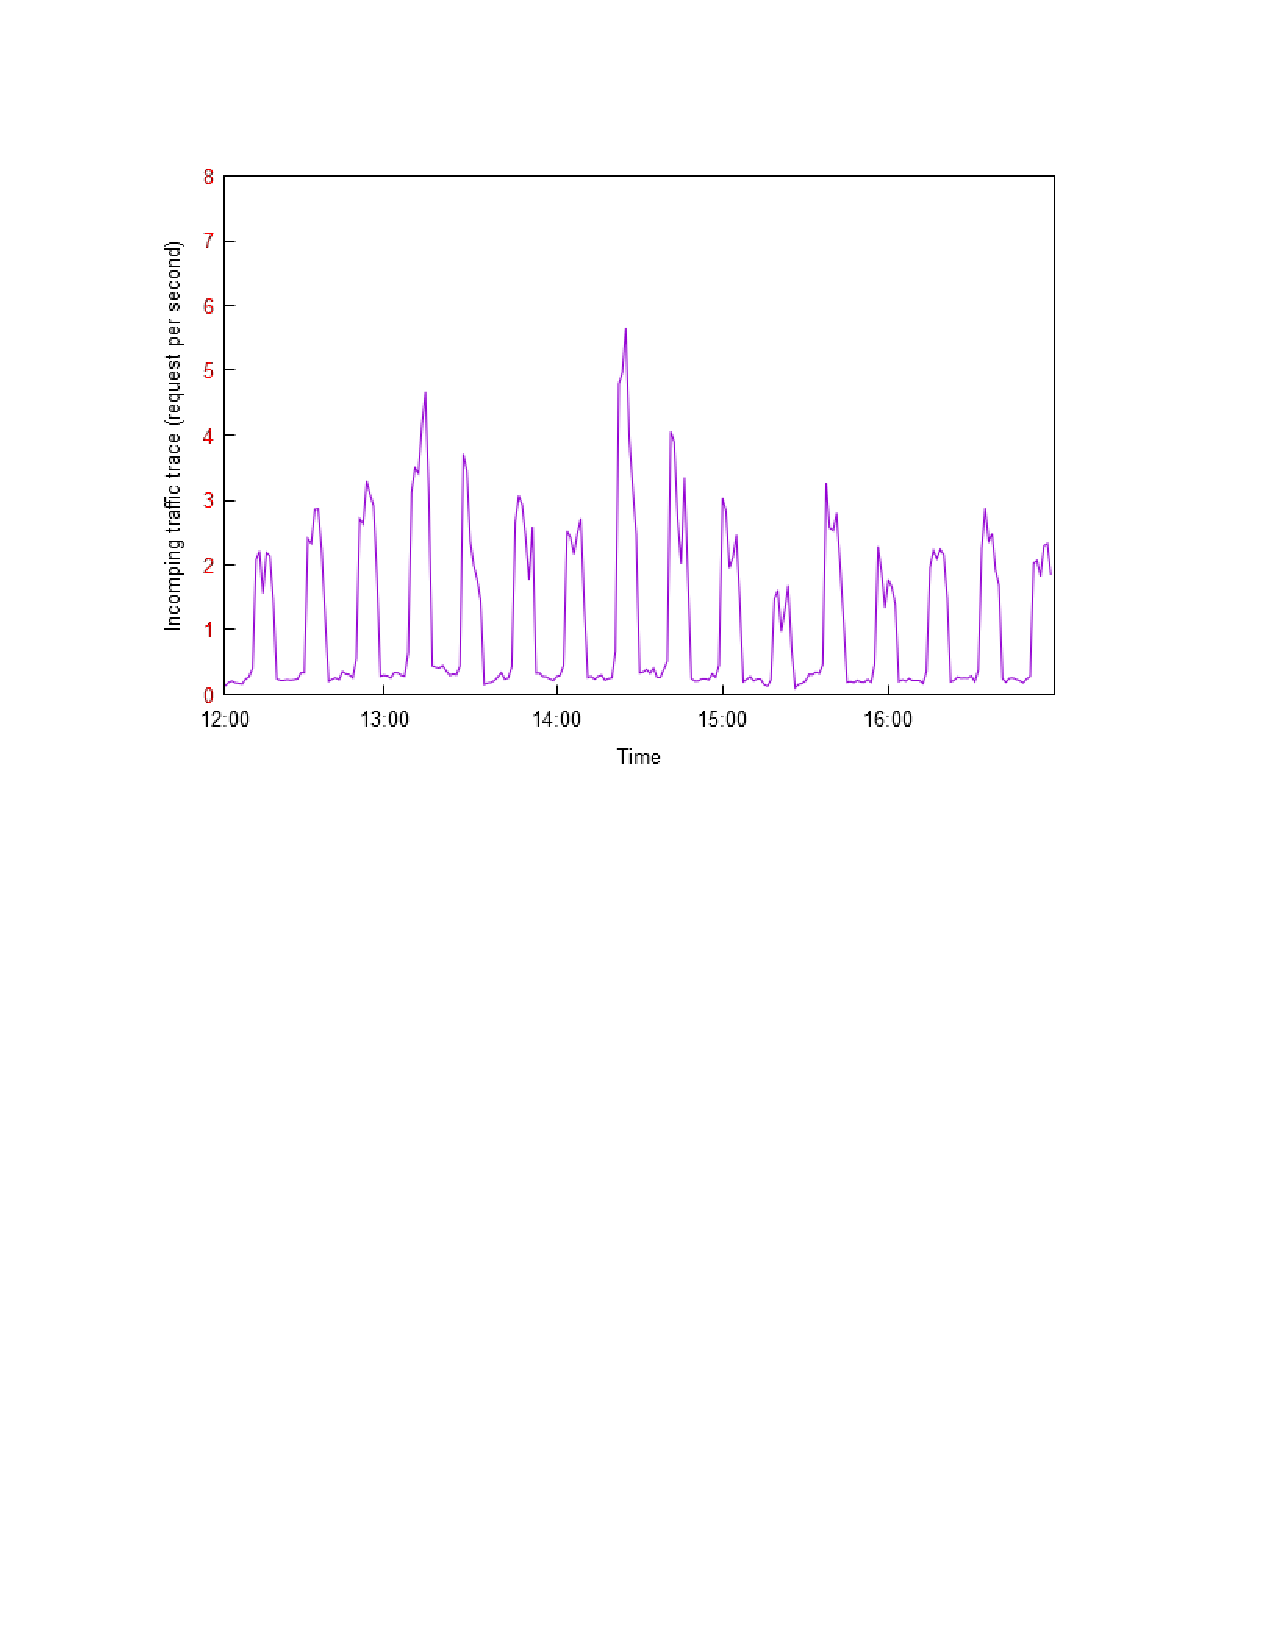
\includegraphics[clip, trim=2.5cm 15cm 3.6cm 2.5cm, width=\columnwidth]{figures/pdf/traffic-2.pdf}
			\caption{4 hours of MAWI trace data of 2017/04/12}
		\end{subfigure}	
		\caption{MAWI traffic trace as input workload}
		\label{fig:traffic}
\end{figure}

\par With the regards of augmented reality for autonomous driving\cite{wintersberger2019fostering,feng2018augmented}, this paper assumes AR service defined with the following attributes as a continuously running service on each vehicle: (i) The size of services is U (50; 500) MB for typical Linux containers\cite{montero2017extending} with the requests have a delay threshold of 10 ms \cite{byers2017architectural}.(ii) The average size of service request and response are U (10; 26) KB and U (10; 20) byte, respectively\cite{ha2013impact}. (iii) The required amount of processing for the services is U (50; 200) MI per request\cite{skarlat2017optimized,yousefpour2019fogplan}.

\section{Conclusion}
we motivate the reader to consider other constraints such as the availability of resources, the reliability of services, etc.\\

\begin{tabular}{l@{$\dots\dots$}p{10cm}}
GSMA\dotfill&Global System for Mobile Communications \\
ITU\dotfill&International Telecommunication Union\\
GeSI\dotfill&Global Enabling Sustainability Initiative\\
SBTi\dotfill&Science Based Targets initiative\\
\end{tabular}

\bibliographystyle{plain}
\bibliography{mybib}

\end{document}


